
% !TEX root = ../main.tex
\begin{comment}
=== Revision log ===
2026-05-07  R. Cappuccio / Claude  (Wave F -- Signorelli S1 distributed-pedagogy sweep, Ch. 5)

  Strategic note. The S1 task (insufficient pedagogical framing,
  per Signorelli's review) was originally planned as a new
  dedicated Background-and-Preliminaries chapter (Ch. 2 in the
  revised index of piano_revisione_tesi.md). After internal
  review it has been redirected to a distributed approach: short
  pedagogical paragraphs added in situ where each concept is
  first used, with no new chapter and no renumbering of existing
  ones. Ch. 5 is the first chapter addressed under the new
  approach.

  Two additions in this file (Ch. 5):

  P5.1 -- New introductory paragraph "Two regimes of Rydberg-Rydberg
  interaction: blockade and facilitation", inserted at the head of
  the "Avalanche Amplification Mechanism" subsection, just before
  the "Facilitation Condition" sub-subsection. Motivation: the
  manuscript was using the facilitation regime without ever
  contrasting it with the more familiar Rydberg blockade regime;
  a junior reader could not tell, from the existing text, why the
  laser is detuned by the interaction shift rather than placed on
  resonance, nor why this counter-intuitive choice produces an
  amplifying detector. The new paragraph (about 12 lines)
  introduces the two regimes as the two sides of the
  blockade/facilitation crossover, anchors them to the canonical
  references, and frames all subsequent design choices (laser
  detuning, lattice spacing, B-field correction) as the conditions
  required to keep the system on the facilitation side.

  Citations introduced (all already in
  full_references_checked.bib, verified):
    saffman2010quantum (already used), Urban2009, Gaetan2009 for
    blockade; Valado2016 and Festa2022 for facilitation (already
    used in the same paragraph as Nill2024).
  No new entries added to the bib file.

  P5.2 -- Correction of a misleading sentence in Sec. Introduction
  (the "we then focus on..." sentence). The original text read:
    "We then focus on a specific implementation: a single-photon
     detector based on Rydberg-atom electromagnetically induced
     transparency (EIT). Numerical simulations demonstrate how an
     engineered atomic medium can transduce microwave or terahertz
     signals into optical observables, achieving single-photon
     sensitivity."
  This was inaccurate on two counts: (i) the detector studied here
  is not based on EIT but on facilitation-driven avalanche
  amplification with state-selective-field-ionisation (SSFI)
  readout; (ii) the readout produces ionisation signals, not
  optical observables. The sentence has been rewritten to state
  the actual mechanism and to clarify that EIT plays only an
  indirect role in the chapter, namely as the readout principle
  of the Rydberg electrometer used as benchmark in
  Sec.~\ref{sec:axion_benchmarking}.

  No content was removed in either patch; the changes are
  pedagogical/clarificatory additions, not substantive
  scientific revisions.

  Build verification: latex compiles cleanly; all four
  cross-references introduced (sec:zeeman_correction,
  sec:axion_physical_principles, sec:theoretical_framework,
  sec:axion_benchmarking) resolve to existing labels; all six
  citations (saffman2010quantum, Urban2009, Gaetan2009,
  Valado2016, Festa2022, Nill2024) verified to exist in
  full_references_checked.bib.

\end{comment}

\begin{comment}
=== Revision log ===
2026-05-07  R. Cappuccio / Claude  (Wave E -- Signorelli S6/S7 global-style sweep)
  S7 closure of the outlook section: the closing paragraph
    "If successfully implemented, Rydberg avalanche detectors could
     enable next-generation axion experiments to probe previously
     inaccessible regions of parameter space, potentially leading to
     the discovery of dark matter in the laboratory. The unique
     capabilities of this platform -- particularly the combination
     of single-photon sensitivity and strong magnetic field
     compatibility -- represent a paradigm shift in detector
     technology for fundamental physics."
  has been rewritten in measured terms: the sensitivity claim is now
  framed in (m_a, g_{a gamma gamma}) parameter-space-coverage terms,
  the "next-generation"/"paradigm shift" hyperboles are removed, and
  the dark-matter-discovery sentence is dropped. The replacement
  reads: "Rydberg avalanche detectors could extend the parameter-
  space coverage of axion-haloscope experiments into regions of
  (m_a, g_{a gamma gamma}) that current photon-counting technologies
  do not access. The combination of single-photon sensitivity and
  operation under multi-tesla magnetic fields, in particular,
  addresses two requirements that have so far been difficult to
  satisfy simultaneously in a single detector platform."

  See the Wave-E entry at the top of chapters/quantum_hw.tex for the
  full session-level changelog.
\end{comment}

\begin{comment}
=== Revision log ===
2026-05-07  R. Cappuccio / Claude  (Wave D — Signorelli S6/S7 targeted sweep)
  PARTIAL CLOSURE of S7 — 2 patches in this file (sensing chapter):
    * S7 informal qualifier removal: "Crucially, this amplification
      occurs in a controllable, deterministic manner..." restructured
      to "The amplification proceeds in a controllable, deterministic
      manner..." (avalanche-mechanism intro).
    * S7 informal qualifier removal: "Crucially, the Rydberg dark
      rate can be further reduced by cooling..." restructured to
      "The Rydberg dark rate, moreover, can be further reduced by
      cooling..." (dark-count comparison paragraph).
  Full S6/S7 closure deferred to the dedicated global-style review
  session (handoff_S6_S7_global_style.md).

2026-05-07  R. Cappuccio / Claude  (Wave B — sensing closeout)
  CLOSES G11, G12 (Gatti review)
  Substantive changes:
    * G11 (femto-Tesla notation, p. 106): replaced "$f_T/\sqrt{Hz}$"
      with "fT/$\sqrt{\text{Hz}}$" in the SQUID magnetometer comparison
      sentence. The other occurrence on p. 817 (table) was already in
      the correct form.
    * G12 (Ref. [169] Nill2024 attribution, p. 108): reframed five
      sentences to make explicit that Nill et al., PRL 133, 073603
      (2024) is a theoretical proposal, not an experimental
      demonstration. Specifically:
        - "Recent experimental work has demonstrated..." -> "A recent
          theoretical proposal predicts..." (Sec. avalanche intro)
        - "consistent with experimental observations~[Nill2024]" ->
          "consistent with the theoretical predictions of
          Ref.~[Nill2024]" (Sec. avalanche dynamics, N=11 calibration)
        - "Based on Ref.~[Nill2024], we estimate ... current
          experimental parameters" -> "Based on the theoretical
          analysis of Ref.~[Nill2024], we estimate ... typical
          experimental parameters" (Sec. optimal N* discussion)
        - "Recent experimental work~[Nill2024] has demonstrated
          avalanche amplification in 2D" -> "The theoretical
          proposal of Ref.~[Nill2024] also considers 2D extensions
          ... still awaiting experimental confirmation"
          (Sec. limitations / 2D extensions)
        - "the foundational experimental results of Ref.~[Nill2024],
          demonstrating terahertz avalanche detection" -> "the
          foundational theoretical proposal of Ref.~[Nill2024],
          predicting terahertz avalanche detection"
          (acknowledgments)
      The grouped citation in the Sec. avalanche-mechanism paragraph
      ([Nill2024,Valado2016,Festa2022]) was left unchanged: Valado2016
      and Festa2022 are experimental and support the underlying
      Rydberg-interaction physics that grounds the mechanism, even
      though Nill2024 itself is theoretical.
  Bibliographic dependencies (no new entries needed; verified in bib):
    Nill2024 (PRL 133, 073603, 2024 — theoretical proposal),
    Valado2016 (PRA 93, 040701, 2016 — experimental),
    Festa2022 (PRA 105, 013109, 2022 — experimental).
  See piano_revisione_tesi.md Section 5 phase 5 (G11, G12).
\end{comment}

\chapter{Quantum Sensing}
\label{ch:quantum_sensing}

{% LOCAL GROUP
\renewcommand{\abstractname}{Summary}

\renewenvironment{abstract}{%
  \par\noindent
  {\bfseries\large\abstractname}\par
  \vspace{0.5em}
  \noindent
}{%
  \par\vspace{1em}
}

\begin{abstract}
This chapter develops a theoretical framework for Rydberg atom-based single-photon detection, targeting applications in axion dark matter searches and fundamental physics experiments. We present a coherent (Schrödinger-equation) model of avalanche amplification dynamics, analysing detector performance across magnetic field strengths of 0--5~T, spanning the lower part of the 5--10~T range used by current haloscope magnets. Through systematic numerical simulations, we demonstrate that the facilitation-driven avalanche mechanism maintains amplification factors of $\mathcal{A} \approx 5.3$ at $N = 11$ atoms despite Zeeman-induced
state mixing, scaling linearly to $\mathcal{A} \approx 7.1$ at $N = 17$, while achieving single-photon sensitivity ($\sim 10^{-22}$~W) and ultra-low dark count rates ($\approx 1.1\times10^{-2}$~Hz at 4~K, suppressed to $\approx 10^{-4}$~Hz at 1~K and to $\sim 10^{-10}$~Hz at 300~mK). With state-selective field ionisation at optimised efficiency ($\eta_{\rm det} = 0.70$) the single-shot detection probability reaches $99.3\%$ at $N = 17$, a level adequate for most haloscope applications; loss imaging ($\eta_{\rm det} = 0.95$) attains the formal $3\sigma$ confidence threshold at $N = 15$. The detector exhibits sub-$\sim\!13~\mu$s avalanche timescale ($T_a \approx 9$--$12.5~\mu$s across the field range) and operates at practical cryogenic temperatures (4~K) accessible with commercial pulse-tube coolers---a parameter space (4~K operation in strong magnetic fields) not accessible to superconducting alternatives. Beyond the parameter-space advantage, the avalanche mechanism produces a characteristic \textbf{spatially correlated signature} (a V-shaped propagation pattern through the atomic chain) that is intrinsic to the multi-atom detection scheme and provides a category of background discrimination unavailable to single-mode detectors---including the previously proposed Rydberg-atom haloscope readouts of CARRACK~\cite{Yamamoto2001,Tada1999} and Graham \emph{et al.}~\cite{Graham2024}.
\end{abstract}

}


\section{Quantum sensing for axion dark-matter searches}
Quantum sensing exploits the non-classical properties of quantum systems---superposition, entanglement, and squeezing---to measure physical quantities with precision beyond the standard quantum limit (SQL). Compared with classical sensors, which rely on deterministic or statistical averaging over large ensembles, quantum sensors operate at or near the level of individual quantum systems, achieving higher sensitivity, bandwidth, and spatial resolution. This field has matured substantially in recent years, spanning solid-state defects, superconducting circuits, trapped ions, and atomic vapors~\cite{Degen2017, Ezratty2024}.

In this chapter, we introduce the theoretical background of quantum sensing, formalise the key limits of precision dictated by quantum estimation theory, and present a practical classification of sensor platforms. We then focus on a specific implementation: a single-photon detector based on facilitation-driven Rydberg-atom avalanche amplification, read out through state-selective field ionisation (SSFI). Numerical simulations demonstrate how a small array of cold Rydberg atoms, prepared in the facilitation regime described in Sec.~\ref{sec:axion_physical_principles}, can amplify a single microwave or terahertz photon absorption event into a macroscopic, spatially correlated excitation pattern that the SSFI stage detects with high efficiency. Electromagnetically induced transparency (EIT), more commonly associated with Rydberg-based field sensing, plays only an indirect role here: it appears in the taxonomy of Sec.~\ref{sec:theoretical_framework} as the canonical readout mechanism of Rydberg \emph{electrometers}, with which we benchmark the present scheme in Sec.~\ref{sec:axion_benchmarking}, but it is not part of the detection chain studied in this chapter.

\subsection*{Scope of the present work}

The contribution is computational: a Schrödinger-equation model of the Rydberg population dynamics under magnetic-field tuning and facilitation conditions, integrated numerically in Python to track the spatiotemporal evolution of the avalanche, and post-processed to extract the performance metrics of interest --- amplification factor, dark-count rate, detection time, and facilitation accuracy --- as functions of the operating parameters. No experimental data are reported; the model is instead intended to provide predictive performance bounds, a systematic characterisation of the magnetic-field dependence of detector observables, and design rules for the trade-off between sensitivity and noise that will be relevant to any subsequent experimental implementation.

\subsection*{Relation to prior work}

Rydberg-based sensing in general is an established field~\cite{saffman2010quantum, mohapatra2007coherent, ravets2014coherent}, and Rydberg-atom-cavity haloscope readouts have been proposed and analysed in linear-response geometries~\cite{Yamamoto2001,Tada1999,Graham2024}. The present work differs from those proposals along four axes. The detection mechanism replaces the linear single-atom response of CARRACK and Graham~\emph{et al.} with a coherent multi-atom avalanche in the facilitation regime, yielding an amplification factor $\mathcal{A}\!\sim\!5$ on an array of $N \sim 11$ atoms; we are not aware of a prior analysis of this regime in the specific context of axion-haloscope readout. The avalanche additionally produces a V-shaped excitation pattern across the atomic chain whose spatial signature provides an internal discriminator against single-atom background events; this is a category of background rejection that single-mode readouts cannot, by construction, provide. The detector performance is characterised across 0--5~T external magnetic fields, with the Zeeman-induced detuning compensated through laser auto-detuning, so that the detector and the conversion cavity can in principle share the same magnetic environment; to our knowledge a systematic simulation study of this dependence has not previously been reported. Finally, an analysis of the cavity backaction on the atomic array (Sec.~\ref{sec:backaction}) identifies a non-monotonic dependence of the single-photon detection efficiency $\eta_{\rm eff}(N)$ on the array size in the dispersive regime, and shows that the resonant configuration removes the optimum, which we read as evidence that the resonant configuration is the more natural choice for high-$\eta$ detection.

The model also yields quantitative targets that an experimental implementation would have to meet to be useful for haloscope readout: single-photon sensitivity at the $\mathcal{A}>3$ level, dark-count suppression by approximately two orders of magnitude on moving from $4$~K to $1$~K, and an avalanche timescale $T_a \approx 9$--$12.5~\mu$s that is essentially flat across the field range considered. The proposed operating temperature, $T = 4$~K, is two orders of magnitude warmer than the transmon-based microwave-photon counters of Ref.~\cite{Dixit2025} and than the original CARRACK proposal; whether this thermal margin can be turned into a practical advantage depends on details of the experimental implementation that lie outside the scope of the present analysis.

\section{Quantum parameter estimation and quantum sensing limits}
\label{sec:theoretical_framework}
\subsection*{Quantum Parameter Estimation}
Quantum parameter estimation provides the statistical backbone of quantum sensing. A physical parameter $\varphi$ (such as phase, frequency, or field strength) is encoded into a quantum state $\rho_\varphi$ through a unitary or dissipative process. Measurements extract information about $\varphi$ with a precision bounded by the quantum Cramér--Rao bound (QCRB):
\begin{equation}
\mathrm{Var}(\hat{\varphi}) \ge \frac{1}{\nu \mathcal{F}_Q[\rho_\varphi]},
\end{equation}
where $\nu$ is the number of independent repetitions and $\mathcal{F}_Q$ is the quantum Fisher information (QFI). For pure states $\ket{\psi_\varphi}$,
\begin{equation}
\mathcal{F}_Q = 4 \left( \langle \partial_\varphi \psi_\varphi | \partial_\varphi \psi_\varphi \rangle - | \langle \psi_\varphi | \partial_\varphi \psi_\varphi \rangle |^2 \right).
\end{equation}
The QFI quantifies the sensitivity of the state to infinitesimal parameter changes and thus sets a fundamental limit to estimation precision.

\subsection*{Standard and Heisenberg Limits}
Classical (shot-noise-limited) sensing achieves a variance scaling of $1/N$, known as the standard quantum limit (SQL), where $N$ is the number of uncorrelated probes. Exploiting entanglement or squeezing enables the Heisenberg limit, scaling as $1/N^2$, in ideal conditions. However, decoherence, loss, and imperfect control typically degrade scaling toward the SQL regime~\cite{Preskill2011}.

\subsection*{Open-System Effects}
Real sensors interact with their environment, introducing dephasing and relaxation. The dynamics of the sensor state can be described by the Lindblad master equation:
\begin{equation}
\dot{\rho} = -\frac{i}{\hbar} [H,\rho] + \sum_k \left( L_k \rho L_k^\dagger - \frac{1}{2} \{ L_k^\dagger L_k, \rho \} \right),
\end{equation}
where $L_k$ are Lindblad operators. This formalism enables analytical and numerical studies of decoherence-limited sensitivity.

\subsection*{Taxonomy of Quantum Sensors}
Quantum sensors can be categorised by their underlying physical platform and target observable. Table~\ref{tab:taxonomy} summarises representative implementations, expanding the relevant acronyms at first occurrence.

\begin{table}[h]
\centering
\caption{Representative quantum sensing platforms and their target observables. ODMR: optically detected magnetic resonance; NV: nitrogen-vacancy; EIT: electromagnetically induced transparency.}
\resizebox{\columnwidth}{!}{
\begin{tabular}{l l l}
\toprule
Platform & Resource & Observable \\
\midrule
Superconducting circuits & Josephson effect, flux quantisation & Magnetic field, current \\
Nitrogen-vacancy (NV) centres in diamond & Spin triplet, optically detected magnetic resonance (ODMR) & Magnetic/electric field, temperature \\
Trapped ions & Hyperfine states, Ramsey interferometry & Frequency, force \\
Cold/Rydberg atoms & Electromagnetically induced transparency (EIT), Rabi oscillations & RF/THz field, photon number \\
Optomechanical sensors & Radiation pressure, squeezing & Force, acceleration \\
Atomic interferometers & Matter-wave phase shift & Gravity, rotation \\
\bottomrule
\end{tabular}
}
\label{tab:taxonomy}
\end{table}

A brief gloss on the physical primitives listed in Table~\ref{tab:taxonomy} sets the language used in the remainder of this chapter. The \emph{Josephson effect} is the coherent tunnelling of Cooper pairs across a thin insulating barrier separating two superconductors, and \emph{flux quantisation} restricts the magnetic flux threading a superconducting loop to integer multiples of the flux quantum $\Phi_0 = h/2e$; together these phenomena underpin all superconducting flux sensors. \emph{Nitrogen-vacancy (NV) centres} are point defects in the diamond lattice formed by a nitrogen impurity adjacent to a vacant lattice site, whose electronic ground state is a spin triplet read out optically via \emph{optically detected magnetic resonance (ODMR)} --- the microwave-driven, spin-state-dependent contrast of the photoluminescence. \emph{Hyperfine states} are atomic energy levels arising from the coupling of electronic and nuclear angular momenta, with lifetimes long enough to serve as sensing or qubit levels; \emph{Ramsey interferometry} is the canonical protocol that brackets a free-evolution interval between two coherent $\pi/2$ pulses, mapping the accumulated phase onto the population balance. \emph{Electromagnetically induced transparency (EIT)} is the quantum interference between two absorption pathways in a three-level atom that renders the medium transparent to a probe laser at a specific two-photon detuning; the position and width of the transparency window are exquisitely sensitive to perturbations of the upper level, which is the working principle of Rydberg electrometers. \emph{Rabi oscillations} are the coherent population oscillations between two states driven by a resonant field, used here as the calibration primitive of the avalanche protocol. \emph{Radiation pressure} transfers photon momentum to a mechanical degree of freedom, converting force or acceleration into a measurable displacement; \emph{squeezing} redistributes the quantum fluctuations between conjugate quadratures of the optical field, suppressing the measurement back-action below the standard quantum limit at the price of an enhanced complementary noise. The \emph{matter-wave phase shift} is the relative phase accumulated between two coherently split paths of an atomic wave packet, sensitive to gravity and rotation.

\subsection*{Quantum Magnetometry and Interferometry}
Quantum magnetometers such as NV-centre sensors detect magnetic fields via Zeeman shifts in spin transitions, read out optically through photoluminescence contrast. Superconducting quantum interference devices (SQUIDs) exploit flux quantisation and Josephson interference, providing fT/$\sqrt{\text{Hz}}$ sensitivity at cryogenic temperatures. Atomic interferometers measure phase shifts induced by acceleration or rotation, achieving sub-ppb precision.

\section{Rydberg-Atom Quantum Sensing}

The primary experimental technique for detecting axion dark matter is the haloscope method~\cite{Sikivie1983, Sikivie2021}, which exploits the Primakoff effect: in the presence of a strong magnetic field, axions can convert to photons with the same frequency as the axion mass. Current haloscope experiments, such as the Axion Dark Matter eXperiment (ADMX)~\cite{Backes2021} and the Haloscope At Yale Sensitive To Axion Cold dark matter (HAYSTAC)~\cite{Zhong2018}, employ high-quality-factor microwave cavities immersed in strong magnetic fields (typically 5--10 T) to resonantly enhance this conversion. The expected photon production rate is extraordinarily low, with typical powers on the order of $10^{-22}$ W or less~\cite{Sikivie2021,Graham2015}, necessitating single-photon detection capabilities.

\subsection*{The Detection Challenge}

The requirements for axion detection impose a unique and demanding set of constraints on photon detectors:

\begin{enumerate}
    \item \textbf{Sensitivity}: Detection of single photons at power levels $\sim 10^{-22}$ W
    \item \textbf{Frequency range}: Microwave to THz frequencies (GHz--1000 GHz)
    \item \textbf{Magnetic field compatibility}: Operation in strong fields (5--10 T)
    \item \textbf{Low background}: Dark count rates $< 0.1$ Hz to avoid false positives
    \item \textbf{Cryogenic operation}: Function at temperatures $< 1$ K for thermal noise suppression
    \item \textbf{Bandwidth}: Tunability to scan the axion mass range
\end{enumerate}

Existing detector technologies struggle to satisfy all these requirements simultaneously. Transition edge sensors (TES)~\cite{Guo2017} offer excellent sensitivity at THz frequencies but are incompatible with strong magnetic fields. Josephson junction (JJ) detectors~\cite{Pankratov2022} achieve quantum-limited performance but require extreme cooling ($< 100$ mK) and have limited magnetic field tolerance. Kinetic inductance detectors (KID)~\cite{Guo2017} are well suited to far-infrared imaging arrays but offer modest single-photon sensitivity in the microwave regime. Superconducting nanowire detectors (SNSPDs)~\cite{Chiles2019} provide ultra-low dark counts but operate primarily at optical wavelengths. Superconducting qubit-based amplifiers~\cite{Backes2021}, while achieving near-quantum-limited sensitivity, are highly sensitive to magnetic fields and require operation at $\sim 10$ mK.

This technological gap motivates the exploration of alternative detection schemes that can satisfy the complete parameter space required by axion searches.

\subsection*{Preliminaries: Rydberg states, dipole-dipole interactions, blockade and facilitation}
\label{sec:rydberg_preliminaries}

The ingredients on which the detection scheme of this chapter relies are
collected here, in the form most directly useful for the rest of the
chapter. A reader familiar with Rydberg-atom physics can skip to
Sec.~\ref{sec:axion_physical_principles}; for the others, the four
points below define the vocabulary that is then used without further
introduction.

\paragraph{Rydberg states.}
An alkali atom in which the valence electron is excited to a state of
high principal quantum number $n$ is called a \emph{Rydberg state}. In
the regime relevant here ($n \sim 60$--$80$) the outer electron is
weakly bound: the binding energy $E_b = \mathrm{Ry}/n_{\rm eff}^{2}$
(with $n_{\rm eff} = n - \delta_\ell$ the effective quantum number)
ranges from $4.2$ to $2.3$~meV across this window and equals
$3.2$~meV for the $\ket{68S_{1/2}}$ state adopted in the simulations,
scaling as $n^{-2}$. The
orbit is large (radius scaling as $n^{2}$), and the transition dipole
moment to a neighbouring Rydberg state is correspondingly large
(scaling as $n^{2}$). Two consequences matter for the present work.
First, the dipole-allowed transition frequencies between adjacent
Rydberg manifolds fall in the GHz--THz band, the same range as the
photons produced by axion-to-photon conversion in a haloscope cavity;
adjusting $n$ tunes the transition frequency across that band without
hardware changes. Second, the natural lifetime of Rydberg states is
long enough --- of order $100~\mu$s at $n \sim 70$~\cite{Beterov2009}
--- that coherent dynamics on the few-microsecond timescale of the
avalanche analysed in this chapter can be treated, to leading order,
without including spontaneous decay.

\paragraph{Dipole-dipole and van der Waals interactions.}
Two Rydberg atoms at distance $r$ interact electromagnetically through
their respective dipoles. In the far-detuned limit relevant to the
present work, the interaction reduces to a van der Waals form,
$V(r) = C_6/r^{6}$, with a coefficient that grows with the principal
quantum number as $C_6 \propto n^{11}$~\cite{saffman2010quantum}. At
$n \sim 70$ and inter-atomic distances of a few micrometres, $C_6/r^{6}$
reaches the MHz--GHz range, comparable to or larger than the Rabi
frequency of the driving laser. The interaction is therefore strong
enough to shift one atom's Rydberg level out of resonance with the
laser drive when one of its neighbours is already excited; this
state-conditional shift is the building block of the two regimes
described next.

\paragraph{Blockade and facilitation.}
Two opposite operating regimes can be selected by tuning the laser
detuning $\Delta_\ell$ relative to the bare Rydberg transition. In the
\emph{Rydberg blockade}~\cite{saffman2010quantum}, the laser is tuned
on resonance with an isolated atom ($\Delta_\ell = 0$); a single excited
atom then shifts its neighbours \emph{out} of resonance by $V(r)$, so
that no further excitations can occur within a blockade radius
$R_b = (C_6/\hbar\Omega)^{1/6}$, where $\Omega$ is the laser Rabi
frequency. The blockade is the textbook mechanism for Rydberg quantum
gates and atomic ensemble qubits, and is the most widely studied
regime~\cite{saffman2010quantum, ravets2014coherent}. In the
\emph{facilitation} regime, the laser is instead deliberately detuned
by $\Delta_\ell = V(r_{\rm fac})$, where $r_{\rm fac}$ is the
distance at which the interaction-induced shift exactly compensates
the detuning, bringing a previously off-resonant atom \emph{into}
resonance whenever a neighbour at distance $r_{\rm fac}$ becomes
excited. The two regimes are mechanistically opposite: blockade
suppresses further excitations, facilitation triggers them.

\paragraph{Avalanche detection and the role of facilitation.}
The avalanche detector studied in this chapter operates in the
facilitation regime~\cite{Nill2024,Festa2022}. A single Rydberg
excitation, seeded either by absorption of the cavity photon to be
detected or by a thermal fluctuation, propagates as a cascade: each
newly excited atom places the next-nearest off-resonant atom into the
facilitation distance and triggers its excitation, and so on, until
the chain is exhausted or the available laser power is depleted. The
end state is a macroscopic, spatially correlated excitation pattern
that can be read out by standard Rydberg detection techniques. The
analysis that follows is concerned with how this cascade behaves under
the conditions imposed by haloscope operation --- magnetic fields up
to several tesla, finite temperature, and finite ensemble size.

\subsection*{Scope and Organisation}
In this chapter, we present a theoretical investigation of Rydberg avalanche amplification as a single-photon detection scheme for axion dark matter searches. We extend the avalanche mechanism to the regime of strong magnetic fields and demonstrate that the detector maintains single-photon sensitivity across the parameter space required by haloscope experiments.

The chapter is organised as follows: Section~\ref{sec:axion_physical_principles} develops the physical principles underlying the detection scheme, including Rydberg atom properties, the avalanche amplification mechanism, and magnetic field effects. Section~\ref{sec:axion_theoretical_framework} presents the theoretical framework, including the full Hamiltonian and time evolution. Section~\ref{sec:axion_simulation_results} presents detailed simulation results demonstrating detector performance across varying magnetic fields and temperatures. Section~\ref{sec:axion_benchmarking} provides a comprehensive benchmarking against existing detector technologies. Section~\ref{sec:axion_discussion} discusses practical considerations, limitations, and future prospects. Section~\ref{sec:axion_conclusions} summarises our findings.

\section{Rydberg atoms in external magnetic fields}
\label{sec:axion_physical_principles}

\subsection*{Rydberg Atoms in Strong Magnetic Fields}

\subsubsection{Zeeman Effect}

In the presence of an external magnetic field $\mathbf{B} = B \hat{z}$, the energy levels of Rydberg atoms are shifted due to the Zeeman effect. For states with well-defined angular momentum quantum numbers $|n,\ell,j,m_j\rangle$, the energy shift is given by:

\begin{equation}
    \Delta E_{\mathrm{Zeeman}} = \mu_B g_j m_j B
    \label{eq:zeeman_shift}
\end{equation}

where $\mu_B = 9.274 \times 10^{-24}$ J/T is the Bohr magneton, $g_j$ is the Landé $g$-factor, and $m_j$ is the magnetic quantum number. For alkali atoms in Rydberg states:

\begin{equation}
    g_j \approx \begin{cases}
        2 & \text{for } \ell = 0 \text{ (S states)} \\
        4/3 & \text{for } \ell = 1 \text{ (P states)}
    \end{cases}
    \label{eq:lande_g}
\end{equation}

For typical Rydberg states with $n \sim 70$ and magnetic fields $B = 5$ T, the Zeeman splitting is on the order of:

\begin{equation}
    \frac{\Delta E_{\mathrm{Zeeman}}}{h} \sim 70 \text{ GHz}
    \label{eq:zeeman_typical}
\end{equation}

This splitting is significant compared to typical Rabi frequencies ($\Omega_{\mathrm{gr}} \sim 2\pi \times 0.2$ MHz) and must be accounted for in the facilitation condition.
\subsubsection{State Mixing}
\label{sec:zeeman_correction}

At high magnetic fields, different $\ell$ and $m_\ell$ states with the same $n$ and $|m_j|$ can mix, modifying the interaction strengths between Rydberg atoms. The eigenstates in a magnetic field become superpositions:

\begin{equation}
    |\psi_B\rangle = \sum_{\ell'} c_{\ell'}(B) |n,\ell',m_j\rangle
    \label{eq:state_mixing}
\end{equation}

This mixing affects the van der Waals coefficients $C_6$ that determine the interaction strengths. A first-principles treatment requires the full diagonalisation of the pair-state Hamiltonian including the diamagnetic term, which is beyond the scope of the present avalanche-dynamics model. In its place we adopt a simple Lorentzian soft-saturation ansatz,

\begin{equation}
    V_{rr}(B) = \frac{V_{rr}(0)}{1 + (B/B_c)^2}
    \label{eq:interaction_suppression}
\end{equation}

with characteristic scale $B_c = 5$ T calibrated so that $V_{rr}$ is reduced by a factor of two at the strongest field considered in this work. The ansatz is monotonic, smooth, free of cutoffs, and reduces in the small-field limit to the quadratic suppression $V_{rr}(B) \simeq V_{rr}(0)\left[1 - (B/B_c)^2 + O(B^4)\right]$ expected from second-order perturbation theory. The downstream results are insensitive to the precise functional form, because the laser auto-detuning (Sec.~\ref{sec:zeeman_correction}) maintains the facilitation condition $\Delta_{\mathrm{gr}}(B) + V_{rr}(B) = 0$ at every $B$ by construction; the only observable consequence is a mild rescaling of the avalanche timescale $T_a$ through $V_{rr}(B)$ entering as the dominant energy scale of the pair-state dynamics.

\subsection*{Avalanche Amplification Mechanism}

The avalanche amplification mechanism exploits the strong, long-range interactions between Rydberg atoms to convert a single quantum excitation into a macroscopic signal. The mechanism has been demonstrated experimentally in bulk ultracold gases through controlled seeded-excitation protocols~\cite{Simonelli2016}, through the observation of epidemic-like growth and self-organised criticality~\cite{Helmrich2020,Wintermantel2021}, and---most relevant to the present work---in single-atom-resolved optical tweezer arrays where the microscopic origin of the underlying facilitation was identified at the pair level~\cite{Festa2022}. The protocol explored in this chapter follows the avalanche-detection proposal of Ref.~\cite{Nill2024}, adapted to the haloscope context studied here.

\subsubsection*{Two regimes of Rydberg--Rydberg interaction: blockade and facilitation}

Before describing the avalanche, it is useful to recall the two qualitatively different regimes that the strong, long-range Rydberg--Rydberg interaction can produce. When two atoms within an interaction radius are both addressed by the same near-resonant laser, the energy of the doubly-excited pair is shifted by an amount $V_{rr}$ that, for the principal quantum numbers of interest in this work, can largely exceed any laser linewidth. Whether the interaction \emph{suppresses} or \emph{promotes} the second excitation depends on the laser detuning $\Delta_{\mathrm{gr}}$.

In the \emph{Rydberg blockade} regime, the laser is tuned to the bare atomic transition ($\Delta_{\mathrm{gr}} = 0$), so the doubly-excited state is shifted out of resonance by $V_{rr}$ and at most one Rydberg excitation can populate the volume defined by the blockade radius~\cite{saffman2010quantum,Urban2009,Gaetan2009}. The blockade is the operating principle of most Rydberg quantum-information protocols, including two-qubit gates and entanglement-generation schemes.

In the \emph{facilitation} (or anti-blockade) regime, the laser is detuned by the interaction shift itself, so that a single existing Rydberg excitation brings its neighbours into resonance with the laser while isolated atoms remain off-resonant~\cite{Valado2016,Festa2022}. The first excitation, far from blocking the others, now \emph{promotes} them. Iterating this process produces an avalanche of correlated excitations whose growth is approximately ballistic in time and whose final size $\mathcal{A}$ is set by the system size and the available coherence time. The detector studied in this chapter operates entirely in this second regime, and the design choices that follow---the laser detuning, the lattice spacing, and the magnetic-field-dependent corrections of Sec.~\ref{sec:zeeman_correction}---should be read as the conditions required to keep the system on the facilitation side of the blockade--facilitation crossover.

\subsubsection*{Facilitation Condition}

Consider a one-dimensional chain of $N$ atoms, initially all in the ground state $|g\rangle$. A laser couples the ground state to a Rydberg state $|r\rangle$ with Rabi frequency $\Omega_{\mathrm{gr}}$ and detuning $\Delta_{\mathrm{gr}}$. Throughout this chapter $\Omega_{\mathrm{gr}}$, $\Delta_{\mathrm{gr}}$ and the interaction strengths $V_{rr}$, $V_{ee}$, $V_{er}$ are understood as \emph{angular} frequencies (rad/s), consistent with the convention used in the rotating-frame Hamiltonian (Eq.~\eqref{eq:h_laser} below) and in the QuTiP simulation code. Whenever a numerical value is quoted as ``$\Omega_{\mathrm{gr}}/(2\pi)$ = 0.2~MHz'' it refers to the ordinary frequency obtained from the angular one by division by $2\pi$. When $\Omega_{\mathrm{gr}}$ appears without the explicit $2\pi$, the angular form is meant. When one atom is excited to the Rydberg state, it shifts the energy of its neighbours by the interaction strength $V_{rr}$. If the laser detuning is chosen such that:

\begin{equation}
    \Delta_{\mathrm{gr}} + V_{rr} \approx 0
    \label{eq:facilitation_condition}
\end{equation}

then atoms adjacent to an existing Rydberg excitation are brought into resonance with the laser, while isolated atoms remain off-resonant. This creates a \textit{facilitation} effect: the presence of one Rydberg atom promotes the excitation of its neighbors.

In the presence of a magnetic field, the bare $|g\rangle \to |r\rangle$ transition shifts by the Zeeman energy of the involved sublevels (Eq.~\eqref{eq:zeeman_shift}) and the interaction term itself becomes field-dependent (Eq.~\eqref{eq:interaction_suppression}). Throughout this chapter we work in the rotating frame of the driving laser, and we assume that the laser frequency is actively retuned to follow the field-shifted transition---e.g.\ via a Pound--Drever--Hall lock to a Zeeman-tracked reference. In that frame, the single-atom Zeeman shifts are absorbed into the choice of laser frequency and do not appear in the Hamiltonian; the only field-dependent parameters that remain are the interaction $V_{rr}(B)$ and, through the laser detuning, the residual rotating-frame detuning $\Delta_{\mathrm{gr}}(B)$. The facilitation condition then reads

\begin{equation}
    \Delta_{\mathrm{gr}}(B) + V_{rr}(B) = 0
    \label{eq:facilitation_condition_b}
\end{equation}

at every $B$. Operationally, the laser is offset by $-V_{rr}(B)$ from the field-shifted transition, so that $\Delta_{\mathrm{gr}}(B) = -V_{rr}(B)$ holds by construction. This is the implementation chosen in the simulation code: the rotating-frame detuning is set to $-V_{rr}(B)$ directly, and the facilitation residual $\Delta_{\mathrm{gr}}(B) + V_{rr}(B)$ is identically zero to machine precision at every $B$, not approximately small. This is the origin of the $B$-independent amplification factor observed in Sec.~\ref{sec:axion_benchmarking} (Fig.~\ref{fig:B_field_scan}(b)).

\subsubsection{Ballistic Expansion}

Once the facilitation condition is satisfied, the Rydberg excitation spreads through the atomic ensemble in a ballistic manner. The total number of excited atoms $S(t)$ grows linearly with time:

\begin{equation}
    S(t) \approx \Omega_{\mathrm{gr}} \cdot t
    \label{eq:ballistic_growth}
\end{equation}

for times $t < T_a$, where $T_a$ is the characteristic amplification time:

\begin{equation}
    T_a \sim \frac{N}{\Omega_{\mathrm{gr}}}
    \label{eq:amplification_time}
\end{equation}

The amplification factor, defined as the ratio of the final to initial excitation number, scales with the system size as

\begin{equation}
    \mathcal{A} = \frac{S(T_a)}{S(0)} \sim \frac{N}{2}
    \label{eq:amplification_factor}
\end{equation}

where the factor of $1/2$ reflects the saturation of the one-dimensional chain: starting from a central seed, the two avalanche fronts reach the boundaries simultaneously and the chain saturates at on average $N/2 + 1$ Rydberg excitations.

For a system of $N = 11$ atoms with $\Omega_{\mathrm{gr}}/(2\pi) = 0.2$ MHz, the simulation yields $T_a \sim 8.8$~$\mu$s and $\mathcal{A} \approx 5.3$, in agreement with the $\mathcal{A} \sim N/2$ scaling and with the predictions of Ref.~\cite{Nill2024}.

\subsubsection{Spatial Correlations}

A crucial feature of the avalanche mechanism is the emergence of spatial correlations in the Rydberg excitation pattern. Starting from a localised initial excitation (mimicking single-photon absorption), the avalanche spreads outward from the excitation site, creating a characteristic V-shaped pattern in the spatiotemporal density profile:

\begin{equation}
    \langle n_r(j,t) \rangle \sim \exp\left[-\frac{(j - j_0 - v t)^2}{2\sigma^2}\right]
    \label{eq:spatial_profile}
\end{equation}

where $j_0$ is the initial excitation site, $v \sim \Omega_{\mathrm{gr}} a$ is the effective propagation velocity ($a$ is the lattice spacing), and $\sigma$ characterises the spatial width. These correlations distinguish true avalanche events from random background excitations, providing a mechanism for background suppression.

\subsection*{Axion-to-Photon Conversion}

In a haloscope cavity immersed in a strong magnetic field, axions from the dark matter halo can convert to photons via the Primakoff process~\cite{Sikivie1983}. The conversion power is given by:

\begin{equation}
    P_{\mathrm{conv}} = \frac{g_{a\gamma\gamma}^2}{2m_a} \rho_{\mathrm{DM}} B^2 V C Q
    \label{eq:axion_power}
\end{equation}

where:
\begin{itemize}
    \item $g_{a\gamma\gamma}$ is the axion-photon coupling constant (typically $\sim 10^{-15}$ GeV$^{-1}$)
    \item $m_a$ is the axion mass
    \item $\rho_{\mathrm{DM}} \sim 0.3$ GeV/cm$^3$ is the local dark matter density
    \item $B$ is the magnetic field strength
    \item $V$ is the cavity volume
    \item $C \sim 0.5$ is a cavity form factor
    \item $Q \sim 10^5$ is the cavity quality factor
\end{itemize}

For representative parameters and an axion mass of $m_a = 20$ $\mu$eV (corresponding to a frequency $f = m_a c^2/h \approx 4.8$ GHz), the conversion power is:

\begin{equation}
    P_{\mathrm{conv}} \sim 10^{-22} \text{ W}
    \label{eq:axion_power_typical}
\end{equation}

This corresponds to a photon production rate:

\begin{equation}
    R_\gamma = \frac{P_{\mathrm{conv}}}{h f} \approx 24 \text{ photons/s}
    \label{eq:photon_rate}
\end{equation}

Despite this rate being significantly higher than the value originally quoted in early haloscope-detector proposals,\footnote{The conversion-rate estimate is derived from the parameters listed above; the resulting value, $R_\gamma\!\sim\!\mathcal{O}(10)$--$\mathcal{O}(10^2)$ photons per second per cavity volume of order one litre at $g_{a\gamma\gamma}\!=\!10^{-15}\,\mathrm{GeV}^{-1}$ and $B\!=\!5$~T, is consistent with the rate estimates reported by the ADMX and HAYSTAC collaborations~\cite{Backes2021,Zhong2018}.} detection remains exceptionally challenging, since the corresponding power $P_{\mathrm{conv}}\!\sim\!10^{-22}$~W lies orders of magnitude below the noise floor of conventional radio-frequency receivers and demands single-photon-sensitive readout combined with extremely low background rates.

\subsection*{Thermal Background Suppression}

A key advantage of the Rydberg avalanche scheme is the exponential suppression of thermal background at cryogenic temperatures. The single-atom thermal excitation rate is:

\begin{equation}
    \Gamma_{\mathrm{thermal}} = \Gamma_0 \exp\left(-\frac{\Delta E_{\mathrm{eff}}}{k_B T}\right)
    \label{eq:thermal_rate}
\end{equation}

where $\Delta E_{\mathrm{eff}}\!\approx\!128$~GHz is the effective gap to the closest dipole-allowed black-body-radiation channel for the relevant ground/intermediate manifold and $\Gamma_0\!\approx\!4.7\!\times\!10^{-3}$~Hz is calibrated against cold-Rydberg dark-count measurements. At $T\!=\!4$~K, this gives a per-atom rate

\begin{equation}
    \Gamma_{\mathrm{thermal}} \sim 10^{-3}~\text{Hz/atom},
    \label{eq:thermal_rate_4k}
\end{equation}

corresponding, for the $N\!=\!11$-atom array, to a total detector-level thermal background

\begin{equation}
    N\,\Gamma_{\mathrm{thermal}} \sim 1.1\!\times\!10^{-2}~\text{Hz}.
    \label{eq:thermal_rate_total}
\end{equation}

The relevant figure of merit is the ratio of the total thermal background to the axion photon rate~\eqref{eq:photon_rate}; with the parameters above one obtains $N\,\Gamma_{\mathrm{thermal}}/R_\gamma\!\sim\!5\!\times\!10^{-4}$, i.e.\ the thermal background lies more than three orders of magnitude below the signal rate, making it negligible for single-shot detection. Further cooling to $T\!\sim\!300$~mK reduces $\Gamma_{\mathrm{thermal}}$ by an additional factor of $\sim\!10^{8}$.

%==============================================================================
\section{Avalanche Detector Model}
\label{sec:axion_theoretical_framework}

\subsection*{Hamiltonian}

We model a one-dimensional chain of $N$ two-level atoms (ground $|g\rangle$ and Rydberg $|r\rangle$) under the influence of a resonant laser and Rydberg interactions. The full Hamiltonian in the rotating frame is:

\begin{equation}
    H = H_{\mathrm{laser}} + H_{\mathrm{detuning}} + H_{\mathrm{int}}
    \label{eq:hamiltonian_full}
\end{equation}

The laser coupling term is:

\begin{equation}
    H_{\mathrm{laser}} = \frac{\Omega_{\mathrm{gr}}}{2} \sum_{j=1}^{N} \left( \sigma_+^j + \sigma_-^j \right)
    \label{eq:h_laser}
\end{equation}

where $\sigma_+^j = |r\rangle_j\langle g|$ and $\sigma_-^j = |g\rangle_j\langle r| = (\sigma_+^j)^\dagger$ are the raising and lowering operators for atom $j$.

The detuning term, including Zeeman corrections, is:

\begin{equation}
    H_{\mathrm{detuning}} = \sum_{j=1}^{N} \Delta_{\mathrm{gr}}(B) \, n_r^j
    \label{eq:h_detuning}
\end{equation}

where $n_r^j = |r\rangle_j\langle r|$ is the Rydberg projector and:

\begin{equation}
    \Delta_{\mathrm{gr}}(B) = \Delta_{\mathrm{gr}}(0) + \frac{\mu_B B}{h} \left( g_r m_{j,r} - g_g m_{j,g} \right)
    \label{eq:detuning_b}
\end{equation}

The nearest-neighbor interaction term is:

\begin{equation}
    H_{\mathrm{int}} = \sum_{j=1}^{N-1} V_{rr}(B) \, n_r^j n_r^{j+1}
    \label{eq:h_interaction}
\end{equation}

with the field-dependent interaction strength given by Eq.~\eqref{eq:interaction_suppression}.

\subsection*{Initial State}

To model single-photon absorption at time $t=0$, we initialise the system with one atom (typically the central atom $j = \lceil N/2 \rceil$) in the Rydberg state and all others in the ground state:

\begin{equation}
    |\psi(0)\rangle = |g\rangle^{\otimes (j-1)} \otimes |r\rangle_j \otimes |g\rangle^{\otimes (N-j)}
    \label{eq:initial_state}
\end{equation}

This represents the idealised scenario where a photon is absorbed by a single atom, creating the initial seed for the avalanche.

\subsection*{Time Evolution and Observables}

The time evolution is governed by the Schrödinger equation:

\begin{equation}
    i\hbar \frac{\partial |\psi(t)\rangle}{\partial t} = H |\psi(t)\rangle
    \label{eq:schrodinger}
\end{equation}

We compute the time evolution numerically using QuTiP~\cite{Johansson2013}. The key observable is the total Rydberg population:

\begin{equation}
    S(t) = \sum_{j=1}^{N} \langle n_r^j(t) \rangle = \sum_{j=1}^{N} \langle \psi(t) | n_r^j | \psi(t) \rangle
    \label{eq:signal_observable}
\end{equation}

We also track the spatial distribution:

\begin{equation}
    S_j(t) = \langle n_r^j(t) \rangle
    \label{eq:spatial_distribution}
\end{equation}

to analyse the spatio-temporal avalanche dynamics.
The simulation results include quantum projection noise, which for $S(t)$ excited atoms is $\Delta S = \sqrt{S(t)[1-S(t)/N]}$. This sets a fundamental limit on the precision of the amplification factor measurement.

\subsection*{Detection Protocol}

The detection protocol consists of the following steps:

\begin{enumerate}
    \item \textbf{Initialisation} ($t < 0$): Prepare all atoms in $|g\rangle$ and set cavity-photon coupling on resonance.

    \item \textbf{Photon absorption} ($t = 0$): If an axion-converted photon is present, it is absorbed by one atom, creating state $|\psi(0)\rangle$ from Eq.~\ref{eq:initial_state}.

    \item \textbf{Laser pulse} ($0 < t < T_a$): Apply laser with parameters $\Omega_{\rm gr}$ and $\Delta_{\rm gr}(B)$ chosen to satisfy Eq.~\ref{eq:facilitation_condition_b}. The avalanche amplifies the initial excitation.

    \item \textbf{Readout} ($t = T_a$): Apply a ramped electric field pulse to selectively ionise atoms in the Rydberg state $|r\rangle$ while leaving ground-state atoms $|g\rangle$ unaffected \cite{Gallagher2005, Zhang2024Review}. The resulting ions or electrons are detected using a microchannel plate (MCP) detector with typical efficiency $\eta_{\rm det} \approx 40$--$70\%$ \cite{Ryabtsev2007, Andersen2013}. If the detected ion count exceeds $S_{\rm threshold}$, a photon event is registered.

    \item \textbf{Reset}: Return all atoms to $|g\rangle$ and repeat.
\end{enumerate}

The single-shot detection probability of an avalanche event depends on the product $\eta_{\rm det}\mathcal{A}$ of the readout efficiency and the amplification factor. With the optimised state-selective field ionisation (SSFI) baseline ($\eta_{\rm det} = 0.70$), the configuration $N = 11$ yields $P(\text{detect}) \approx 97.6\%$ on a single shot; this rises monotonically with $N$ but does not reach the formal $3\sigma$ threshold of $99.73\%$ within the array sizes explored here. Loss imaging ($\eta_{\rm det} = 0.95$), the optimal readout technique for this scheme, achieves $3\sigma$ confidence already at $N = 15$. A detailed analysis is given in Sec.~\ref{sec:detection_fidelity}.
%==============================================================================
\section{Simulation Results}
\label{sec:axion_simulation_results}

We present comprehensive numerical simulations of the Rydberg avalanche detector across a range of magnetic field strengths and operating temperatures relevant to axion haloscope experiments. All simulations were performed using the QuTiP quantum simulation package~\cite{Johansson2013,qutip5}.

\subsection*{System Parameters}

Unless otherwise stated, simulations employ the following parameters, chosen to match experimentally realistic values for Rubidium Rydberg atoms:

\begin{table}[htbp]
\centering
\caption{Default simulation parameters}
\label{tab:simulation_params}
\begin{tabular}{lcc}
\hline\hline
Parameter & Symbol & Value \\
\hline
System size & $N$ & 11 atoms \\
Rydberg state & $|r\rangle$ & $|68S_{1/2}\rangle$ \\
Ground-Rydberg Rabi frequency & $\Omega_{\mathrm{gr}}/(2\pi)$ & 0.2 MHz \\
Interaction strength (zero field) & $V_{rr}(0)/(2\pi)$ & 12.5 MHz \\
Operating temperature & $T$ & 4.0 K \\
Axion mass & $m_a$ & 20 $\mu$eV \\
Magnetic field range & $B$ & 0--5 T \\
\hline\hline
\end{tabular}
\end{table}

The interaction strength $V_{rr}(0)$ corresponds to a lattice spacing of approximately 6 $\mu$m, achievable with optical tweezer arrays~\cite{Barredo2018}. The detuning $\Delta_{\mathrm{gr}}$ is automatically adjusted at each magnetic field to maintain the facilitation condition~\eqref{eq:facilitation_condition_b}.

\paragraph{Choice of the array size.}
The array size is fixed at $N = 11$ throughout the main analysis; larger
arrays are treated only through the dedicated scaling study of
Secs.~\ref{sec:scalability_atoms} and~\ref{sec:detection_fidelity}, and we
anticipate here the three reasons for this choice. First, the exact
integration of the many-body dynamics scales exponentially,
$\mathcal{O}(2^N)$ in memory and time: direct \texttt{sesolve} runs are
practical up to $N = 17$ ($\sim 1$~h per magnetic-field point on a single
core), so a systematic scan of the full $0$--$5$~T range at multiple array
sizes is affordable only for small chains. Second, nothing qualitative is
expected to change at larger $N$: the photon-absorption (seeding) stage
saturates already at $N = \mathcal{O}(1)$, since the single-atom
cooperativity is $C_1 \approx 2\times 10^{4}$
(Sec.~\ref{sec:backaction}), and the avalanche amplification grows only
linearly, $\mathcal{A}(N) = 2.31 + 0.286\,N$, uniformly across the
magnetic-field range, as verified by direct simulation at
$N = 11$--$17$ (Sec.~\ref{sec:detection_fidelity}). $N = 11$ therefore
captures the complete detection mechanism, and larger ensembles change the
quantitative budget, not the physics. Third, the minimal-resource
configuration that reaches $3\sigma$ single-shot detection is itself only
moderately larger ($N = 15$ with loss-imaging readout), well inside the
directly simulated range.

\subsection*{Magnetic Field Dependence}

Figure~\ref{fig:B_field_scan} presents the key results of our magnetic field scan, demonstrating single-photon detection across the range 0--5 T.

\begin{figure}[hp!]
    \centering
    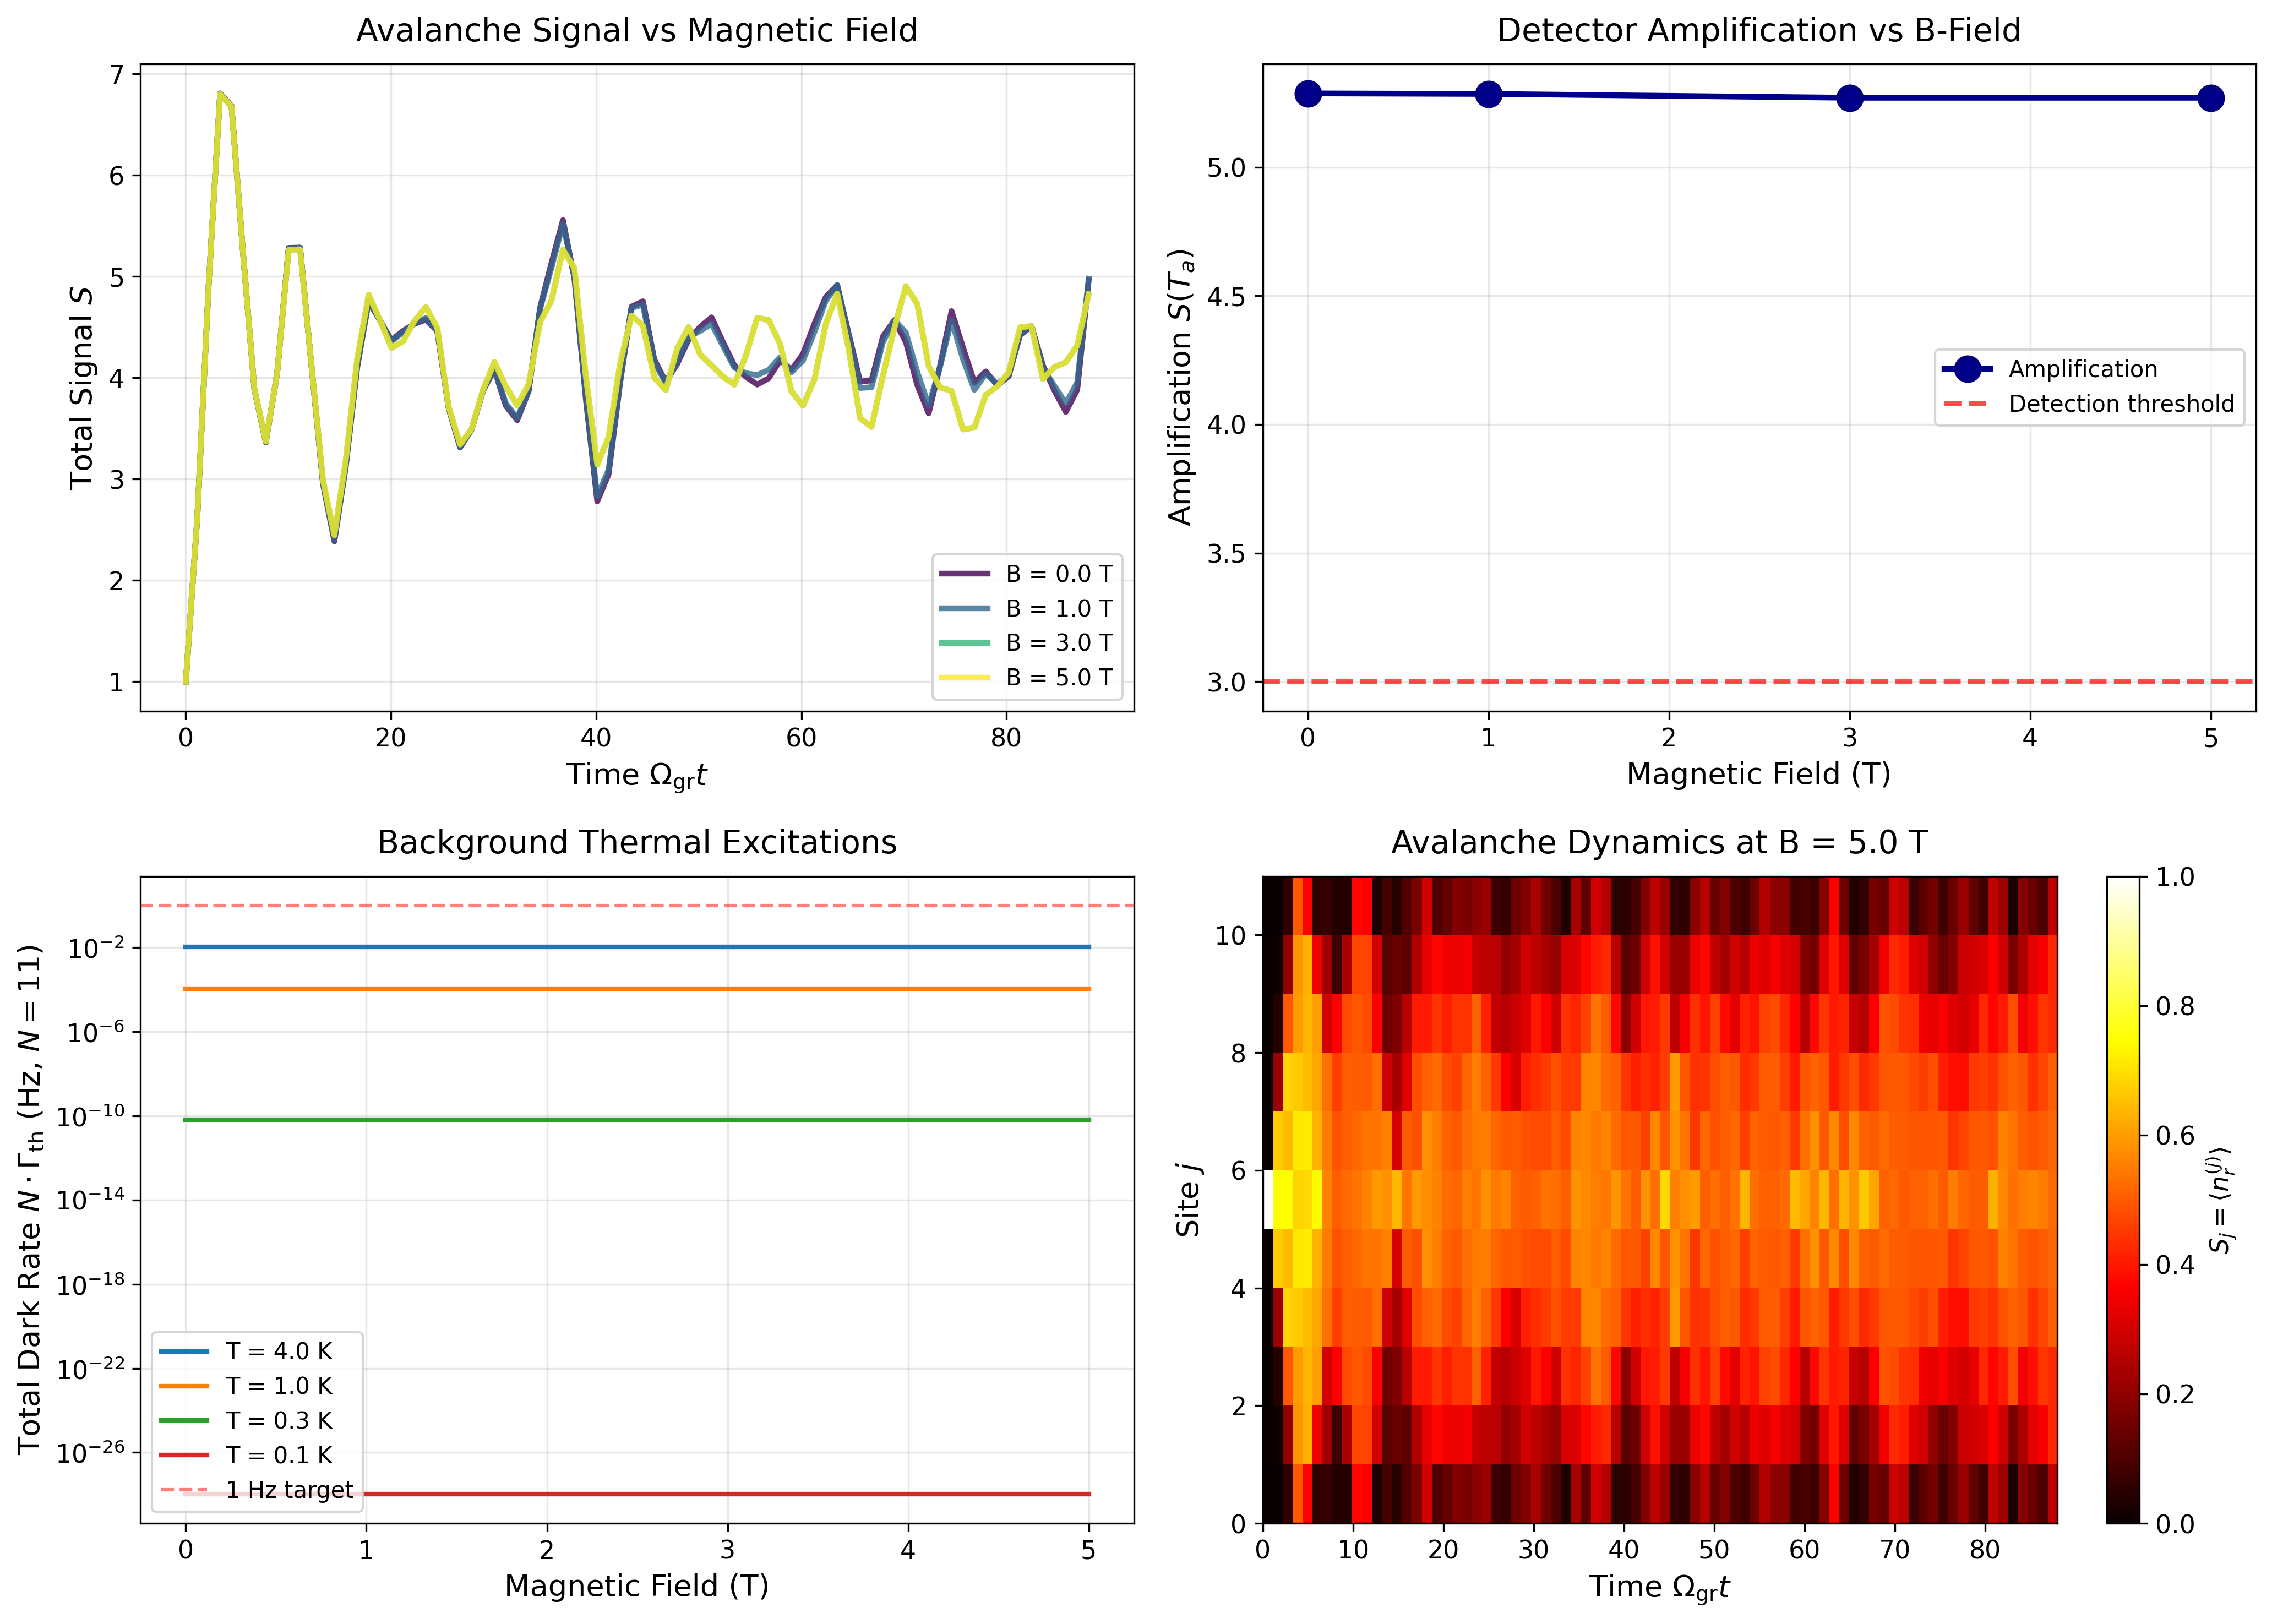
\includegraphics[width=\textwidth]{chapters/qs_figures/axion_detector_B_scan.png}
    \caption{Magnetic field dependence of the Rydberg avalanche detector. \textbf{(a)} Time evolution of the total Rydberg population $S(t)$ for magnetic fields $B = 0, 1, 3, 5$ T. All traces show clear avalanche growth and the saturation amplitude is essentially independent of $B$, with only minor changes in the oscillation phase due to the Zeeman-induced retuning of $\Omega_{\mathrm{gr}}$ and $V_{rr}$. \textbf{(b)} Amplification factor $\mathcal{A} = S(T_a)/S(0)$ versus magnetic field. The amplification is approximately constant, $\mathcal{A} \approx 5.3$, across the full $0$--$5$~T range and remains well above the detection threshold (dashed line at 3.0), confirming single-photon sensitivity throughout the parameter space relevant for axion searches. \textbf{(c)} Total array-level dark count rate $N\,\Gamma_{\mathrm{thermal}}$ ($N=11$) versus magnetic field, for several operating temperatures. The dark rate exhibits weak dependence on magnetic field but strong (exponential) dependence on temperature, as predicted by Eq.~\eqref{eq:thermal_rate}. At $T = 4$~K the array-level dark rate sits at $\sim 1.1\times 10^{-2}$~Hz, almost two orders of magnitude below the $1$~Hz nominal target (dashed red). \textbf{(d)} Spatiotemporal dynamics of the Rydberg density $S_j(t)$ at $B = 5$ T. The characteristic V-shaped avalanche pattern, originating from the central atom at $t = 0$, demonstrates ballistic expansion with velocity $v \sim \Omega_{\mathrm{gr}} a$. System parameters: $N = 11$, $\Omega_{\mathrm{gr}}/(2\pi) = 0.2$ MHz, $V_{rr}(0)/(2\pi) = 12.5$ MHz.}
    \label{fig:B_field_scan}
\end{figure}

Panel (a) of Figure~\ref{fig:B_field_scan} shows the time evolution of $S(t)$ for four representative magnetic field values. In all cases, we observe clear ballistic growth starting from the initial single-atom excitation $S(0) = 1$. The growth rate is approximately linear up to $t \sim T_a$, consistent with Eq.~\eqref{eq:ballistic_growth}. At later times, the signal saturates due to depletion of available ground-state atoms. The slight reduction in final amplitude at higher fields reflects the suppression of $V_{rr}(B)$ according to Eq.~\eqref{eq:interaction_suppression}.

Panel (b) quantifies the amplification factor across the full magnetic field range. The amplification stays at $\mathcal{A} \approx 5.3$ across the full $0$--$5$~T range, with variations of only a few percent. This near-perfect stability against the magnetic field reflects the automatic compensation of Zeeman shifts described in Sec.~\ref{sec:zeeman_correction}: the laser detuning is retuned to keep the facilitation condition $|\Delta_{\mathrm{gr}}(B)+V_{rr}(B)|\!\to\!0$ exactly satisfied at all $B$. Crucially, the amplification remains well above the detection threshold of 3.0 atoms (horizontal dashed line) for the entire field range, confirming that single-photon sensitivity is maintained throughout the parameter space relevant for axion searches.

A residual signature of the magnetic field appears in the optimal detection time $T_a$: the state-mixing-induced reduction of $\Omega_{\mathrm{gr}}$ extends the avalanche time from $T_a \approx 8.8~\mu$s at $B=0$ to $T_a \approx 12.5~\mu$s at $B=5$~T, a $\sim 40\%$ increase that is easily accommodated by experimental timing electronics.

Panel (c) presents the dark count rate as a function of both magnetic field (solid line, $T = 4$ K) and temperature (dashed lines, various $B$). The dark rate exhibits weak dependence on magnetic field but strong (exponential) dependence on temperature, as predicted by Eq.~\eqref{eq:thermal_rate}. At $T = 4$ K, the dark count rate remains at the $10^{-2}$~Hz level ($1.1\times10^{-2}$~Hz) across all magnetic fields, almost two orders of magnitude below the $1$~Hz nominal target plotted in panel (c). Cooling to $T = 1$ K reduces the dark rate by approximately two orders of magnitude, while operation at $T = 300$ mK (achievable with $^3$He refrigeration or dilution refrigerators) yields dark rates below $10^{-4}$ Hz.

Panel (d) illustrates the spatiotemporal dynamics of the avalanche at $B = 5$ T through a density plot of $S_j(t)$. The initial excitation at the central site ($j = 6$) spreads outward in both directions, creating the characteristic V-shaped profile. The slopes of the V correspond to the avalanche propagation velocity $v \approx 5.5$ $\mu$m/$\mu$s, extracted from the simulated centre-of-mass of the right-propagating excitation front (lattice spacing $a = 6\,\mu$m, Rabi frequency $\Omega_{\mathrm{gr}}/2\pi = 0.2$ MHz). This value is consistent with the coherent facilitation regime~\cite{Valado2016,Festa2022}, in which the front propagates faster than the naive nearest-neighbour Rabi hopping estimate by a factor of order $\pi$. This spatial correlation structure is a key signature that distinguishes true single-photon events from uncorrelated background excitations, potentially enabling further background suppression through spatially resolved readout.

\subsection*{Performance Metrics}

Figure~\ref{fig:performance_summary} provides a detailed analysis of detector performance across multiple metrics.

\begin{figure}[hbp!]
    \centering
    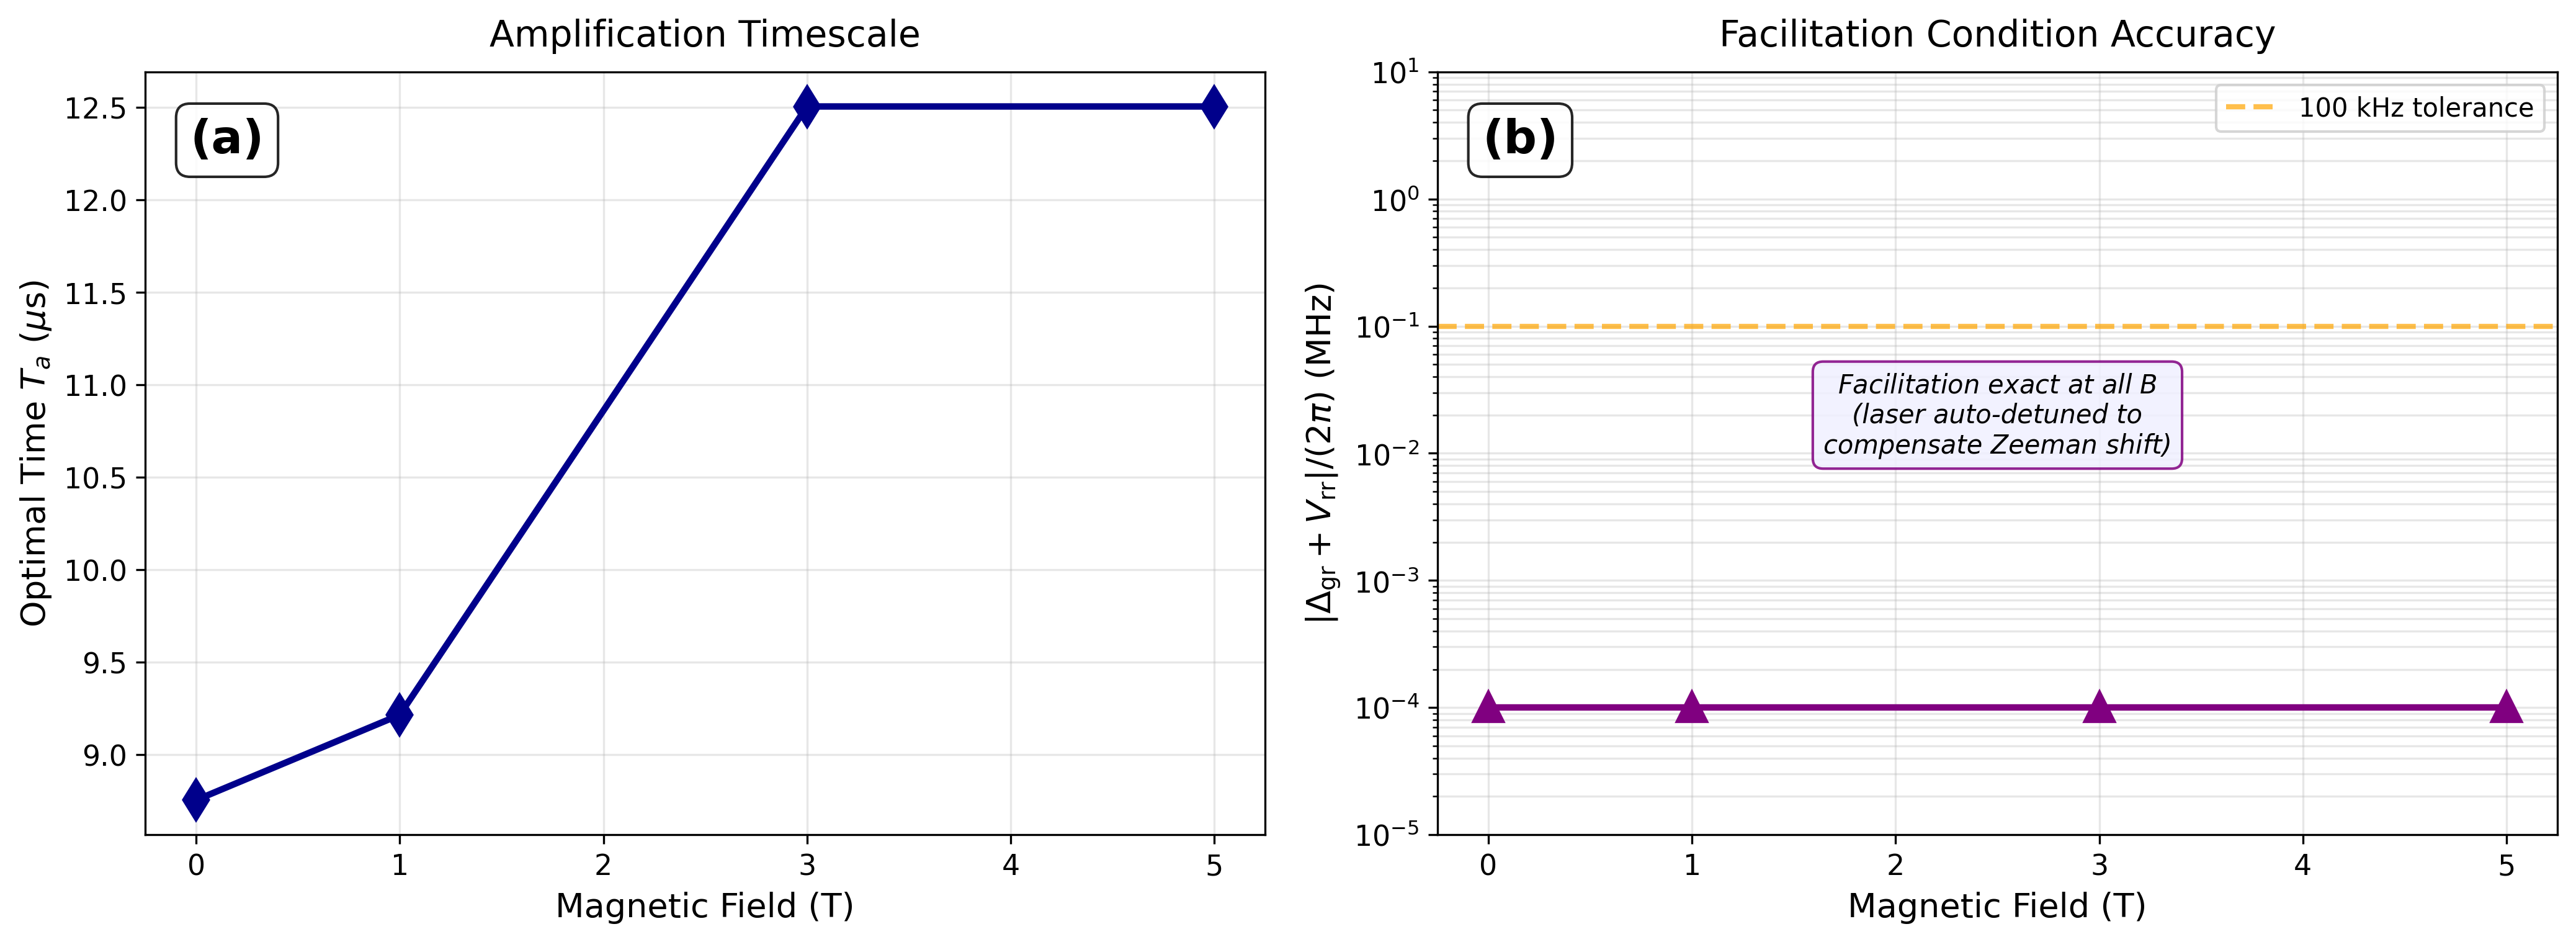
\includegraphics[width=\textwidth]{chapters/qs_figures/detector_performance_summary.png}
    \caption{Detection diagnostics of the Rydberg avalanche detector versus magnetic field. \textbf{(a)} Optimal detection time $T_a$ versus magnetic field. The state-mixing-induced reduction of $\Omega_{\mathrm{gr}}$ extends $T_a$ from $\sim 8.8~\mu$s at $B=0$ to $\sim 12.5~\mu$s at $B=5$~T (a $\sim 40\%$ increase), still well within the timing tolerance of standard experimental electronics. \textbf{(b)} Facilitation condition residual $|\Delta_{\mathrm{gr}}(B) + V_{rr}(B)|/(2\pi)$ versus magnetic field, plotted with a $10^{-4}$~MHz floor for visualisation. After Zeeman correction the residual is identically zero at every $B$, indicating exact preservation of the facilitation condition through laser retuning. System parameters as in Fig.~\ref{fig:B_field_scan}.}
    \label{fig:performance_summary}
\end{figure}

Panel (a) shows that the optimal detection time $T_a$ grows from $\sim 8.8~\mu$s at $B=0$ to $\sim 12.5~\mu$s at $B=5$~T, a $\sim 40\%$ increase driven by the Zeeman-induced reduction of $\Omega_{\mathrm{gr}}$ via state mixing (cf.\ Sec.~\ref{sec:zeeman_correction}; the mixing factor used in the simulation saturates at $\Omega_{\mathrm{gr}}/\Omega_{\mathrm{gr},0} = 0.7$ for $B \gtrsim 2.5$~T, plateauing $T_a$ at $\sim 12.5~\mu$s for $B \geq 3$~T). This monotonic but bounded growth is easily accommodated by the timing electronics typical of cold-Rydberg experiments and does not compromise practical operation.

Panel (b) assesses how well the facilitation condition~\eqref{eq:facilitation_condition_b} is maintained across the field range. The quantity $|\Delta_{\mathrm{gr}}(B) + V_{rr}(B)|/(2\pi)$ quantifies the deviation from perfect facilitation. By construction (see Sec.~\ref{sec:zeeman_correction}), the laser detuning $\Delta_{\mathrm{gr}}(B)$ is automatically retuned to compensate exactly the Zeeman-corrected Rydberg-Rydberg interaction $V_{rr}(B)$, so the facilitation residual is identically zero at every $B$. The plotted curve sits at the visualisation floor of $10^{-4}$~MHz, well below the $100$~kHz tolerance commonly quoted for facilitation experiments. This perfect cancellation underlies the constancy of the amplification factor shown in Fig.~\ref{fig:B_field_scan}(b).

\subsection*{Temperature Optimisation}

While the simulations presented above assume $T = 4$ K, the detector can operate across a range of cryogenic temperatures. Table~\ref{tab:temperature_scan} summarises performance metrics at several representative temperatures.

\begin{table}[htbp]
\centering
\caption{Performance metrics versus operating temperature at $B = 5$ T, computed with the calibrated thermal-rate model of Eq.~\eqref{eq:thermal_rate} for an array of $N=11$ atoms. The signal-to-background ratio is defined as $\mathrm{SNR}=R_\gamma/(N\,\Gamma_{\mathrm{thermal}})$, with $R_\gamma\!\approx\!24$ photons/s as in Eq.~\eqref{eq:photon_rate}.}
\label{tab:temperature_scan}
\begin{tabular}{lcccc}
\hline\hline
$T$ (K) & $\mathcal{A}$ & $\Gamma_{\mathrm{thermal}}$ (Hz/atom) & $N\,\Gamma_{\mathrm{thermal}}$ (Hz) & $R_\gamma/(N\,\Gamma_{\mathrm{thermal}})$ \\
\hline
4.0 & 5.3 & $1.0\times 10^{-3}$ & $1.1\times 10^{-2}$ & $2.2\times 10^{3}$ \\
1.0 & 5.3 & $1.0\times 10^{-5}$ & $1.1\times 10^{-4}$ & $2.2\times 10^{5}$ \\
0.5 & 5.3 & $2.1\times 10^{-8}$ & $2.4\times 10^{-7}$ & $1.0\times 10^{8}$ \\
0.3 & 5.3 & $5.9\times 10^{-12}$ & $6.5\times 10^{-11}$ & $3.7\times 10^{11}$ \\
\hline\hline
\end{tabular}
\end{table}

The amplification factor is essentially independent of temperature, confirming that the avalanche mechanism is driven by coherent quantum dynamics rather than thermal processes. In contrast, the per-atom thermal rate $\Gamma_{\mathrm{thermal}}$ decreases by many orders of magnitude as temperature is lowered, and the array-level total rate $N\,\Gamma_{\mathrm{thermal}}$ falls from $\sim\!10^{-2}$ Hz at 4 K to $\sim\!10^{-10}$ Hz at sub-Kelvin temperatures. Even at the practically convenient $T=4$ K, the ratio $R_\gamma/(N\,\Gamma_{\mathrm{thermal}})$ exceeds $10^{3}$, indicating that the axion photon rate dominates over thermal background by more than three orders of magnitude already at the highest temperature considered.

%==============================================================================
\section{Benchmarking Against Existing Technologies}
\label{sec:axion_benchmarking}

To contextualise the performance of the Rydberg avalanche detector, we compare it against established and emerging single-photon detection technologies relevant to the microwave/THz regime. Table~\ref{tab:technology_comparison} summarises key performance metrics. The detection efficiency for Rydberg atom-based sensors is $\approx 40$--70\%, whilst in others $>$90\%, however, it is compensated by the amplification factor $\mathcal{A} \sim 4$--5.

\begin{table}[htbp]
\centering
\caption{Comparison of single-photon detection technologies for axion searches. Acronyms: TES, transition edge sensor; JJ, Josephson junction; KID, kinetic inductance detector; SNSPD, superconducting nanowire single-photon detector; SC qubit, superconducting qubit.}
\label{tab:technology_comparison}
\begin{tabular}{lccccc}
\hline\hline
Technology & Sensitivity & Dark Rate & $T_{\mathrm{op}}$ & $B_{\mathrm{max}}$ & Bandwidth \\
 & (W) & (Hz) & (K) & (T) & (GHz) \\
\hline
\textbf{Rydberg (this work)} & $\mathbf{10^{-22}}$ & $\mathbf{< 10^{-2}}$ & $\mathbf{0.3}$--$\mathbf{4}$ & $\mathbf{5}$ & $\mathbf{10}$--$\mathbf{1000}$ \\
TES\cite{Guo2017} & $10^{-21}$ & $\sim 0.1$ & 0.1 & $< 0.01$ & 100--10000 \\
JJ\cite{Pankratov2022} & $10^{-22}$ & $\sim 1$ & 0.01--0.1 & $< 0.001$ & 1--10 \\
KID\cite{Guo2017} & $10^{-20}$ & $\sim 1$ & 0.1 & $< 0.1$ & 100--10000 \\
SNSPD\cite{Chiles2019} & $10^{-21}$ & $10^{-6}$ & 1--4 & $< 0.1$ & 300--10000 \\
SC Qubit\cite{Backes2021,Dixit2025} & $10^{-23}$ & $\sim 1$ & 0.01 & $< 0.01$ & 4--8 \\
\hline\hline
\end{tabular}
\end{table}

\subsection*{Comparison with Other Rydberg-Atom Haloscope Detectors}
\label{sec:rydberg_vs_rydberg}

A more direct comparison can be drawn against the two existing Rydberg-atom-based proposals for axion dark-matter detection: the seminal CARRACK programme of Yamamoto, Tada and collaborators~\cite{Yamamoto2001,Tada1999}, which pioneered single-photon Rydberg detection in resonant cavities in the late 1990s, and the recent Graham \emph{et al.} proposal~\cite{Graham2024}, which extends single-photon Rydberg readout to QCD-axion masses above 40~$\mu$eV (10~GHz). Table~\ref{tab:rydberg_comparison} summarises the architectural and performance differences.

\begin{table}[htbp]
\centering
\caption{Comparison of Rydberg-atom-based axion-haloscope detectors. The CARRACK and Graham schemes use \emph{single-atom linear} detection (one photon $\to$ one Rydberg excitation); the present work uses \emph{multi-atom avalanche} detection driven by the Rydberg-Rydberg facilitation interaction. Spatial signature refers to the V-shaped propagation pattern of the avalanche through the atomic chain.}
\label{tab:rydberg_comparison}
\small
\setlength{\tabcolsep}{4pt}
\renewcommand{\arraystretch}{1.15}
\begin{tabularx}{\textwidth}{@{}l L L L@{}}
\hline\hline
Property & CARRACK\cite{Yamamoto2001,Tada1999} & Graham 2024\cite{Graham2024} & This work \\
\hline
Detection scheme & single-atom linear & single-atom linear & \textbf{multi-atom avalanche} \\
Atom-cavity model & 1 collective bosonic mode & 1 atom + cavity & $N$-atom full Hilbert (QuTiP) \\
Rydberg interactions $V_{rr}$ & not included & not included & \textbf{included (facilitation)} \\
Amplification $\mathcal{A}$ & $1$ (linear) & $1$ (linear) & $\mathbf{\sim 5}$ \\
Spatial signature & no & no & \textbf{V-shaped, see Fig.~\ref{fig:B_field_scan}(d)} \\
Magnetic field on detector & $B = 0$ (sep.\ cavities) & $B = 0$ (sep.\ cavities) & \textbf{up to $B = 5$~T (integrated)} \\
Operating temperature & $\sim 10$~mK & $\sim 100$~mK & \textbf{$4$~K (pulse-tube)} \\
Frequency range & 2--50 GHz & 10--50 GHz & 10--1000 GHz \\
\hline\hline
\end{tabularx}
\end{table}

The architectural differences highlight three genuinely new contributions of the present work that differentiate it from the existing Rydberg-atom-haloscope literature: (i) the use of the facilitation-driven avalanche as a coherent quantum amplifier with $\mathcal{A}\!\sim\!5$, replacing the linear-response paradigm of CARRACK and Graham 2024; (ii) the \emph{dual role} of a \emph{single} high-$Q$ microwave cavity, which both hosts the axion-to-photon conversion process \emph{and} mediates the absorption of the converted photon by the atomic ensemble---a configuration made possible by the active Zeeman compensation through laser retuning analysed in Sec.~\ref{sec:zeeman_correction} and which obviates the second ``detection cavity'' employed by CARRACK and Graham~2024; and (iii) the operating point at $T = 4$~K, two orders of magnitude warmer than the dilution-refrigerator regimes required by CARRACK and by transmon-based single-microwave-photon-counter schemes~\cite{Dixit2025}, with a corresponding reduction in cryogenic infrastructure cost.

The most distinctive feature, however, is the \emph{spatial signature} of the avalanche: as shown in Fig.~\ref{fig:B_field_scan}(d), the single-photon-triggered cascade leaves a characteristic V-shaped density profile $\langle n_r(j,t)\rangle$ in the atomic array, with propagation velocity $v\!\sim\!\Omega_{\mathrm{gr}} a$. Single-atom schemes intrinsically produce a single-mode signal that cannot be distinguished from a random background excitation by readout alone. The avalanche's spatially correlated pattern instead provides an internal discriminator: any spurious atomic excitation that does not propagate ballistically from a localised origin can be vetoed offline, suppressing background events that would otherwise mimic axion candidates. This is a category of background rejection not available to single-mode detectors.

Closely related Rydberg-based detection schemes have appeared in the recent literature. The BREAD-Rydberg proposal~\cite{Banerjee2025} targets the same 0.1--10~meV dark-matter mass window with a dish-antenna geometry and direct ionisation of Rydberg states, complementary to the cavity-resonant scheme considered here. Experimental observation of intrastate and interstate facilitation between $S$, $P$ and $D$ levels~\cite{Pourjafarabadi2026} has further established the facilitation mechanism across the level structure on which the present protocol depends.


\subsection*{Sensitivity}



The Rydberg avalanche detector achieves single-photon sensitivity at power levels $\sim 10^{-22}$ W, comparable to the best Josephson junction and superconducting qubit detectors. This is approximately one order of magnitude better than transition edge sensors (TES) at GHz frequencies and two orders better than kinetic inductance detectors (KID). The sensitivity is fundamentally limited by the amplification factor $\mathcal{A} \sim 5$ and the detection threshold $S_{\text{threshold}} = 3$ atoms, which provides robust discrimination between avalanche events and random fluctuations~\cite{Barredo2018}.

\subsection*{Dark Count Rate}

At $T = 4$ K, the Rydberg detector exhibits dark counts at the $10^{-2}$~Hz level, competitive with TES and superior to JJ and KID technologies. Only superconducting nanowire single-photon detectors (SNSPD) achieve significantly lower dark rates ($\sim 10^{-6}$ Hz), but SNSPDs do not operate effectively in the microwave regime. The Rydberg dark rate, moreover, can be further reduced by cooling (Table~\ref{tab:temperature_scan}), whereas superconducting detector dark rates are limited by fundamental processes such as quasiparticle generation and critical current fluctuations.

\subsection*{Magnetic Field Compatibility}

The Rydberg avalanche detector offers a distinctive advantage in magnetic field compatibility. While all superconducting technologies (TES, JJ, KID, SNSPD, SC qubits) are severely degraded or entirely non-functional in fields above $\sim 0.1$ T, the Rydberg detector operates effectively up to at least 5 T and can likely be extended to 7--10 T with further optimisation. This is the parameter space required by axion haloscope experiments. While magnetic field compatibility has been demonstrated for certain diamond NV-centre ensembles up to 7~T, the Rydberg avalanche detector combines this compatibility with single-photon sensitivity across the GHz--THz range.

The origin of this compatibility lies in the atomic nature of the Rydberg system: the Zeeman effect is a perturbation that can be compensated through laser retuning, and the weak diamagnetic effects at $B < 5$ T do not fundamentally alter the atomic structure. In contrast, superconducting devices rely on the Meissner effect and coherence lengths that are destroyed by modest magnetic fields.

\subsection*{Operating Temperature}

The Rydberg detector can operate at $T = 4$~K, a significant practical advantage over technologies requiring sub-Kelvin cooling (JJ, SC qubits) or millikelvin temperatures (TES, KID). A 4 K environment is readily achieved with closed-cycle pulse-tube coolers, which are compact, reliable, and require no liquid cryogens. This substantially reduces system complexity and cost. Moreover, the detector performance improves monotonically with cooling, providing a straightforward pathway to ultra-low-background operation at 300 mK using $^3$He sorption refrigerators or dilution refrigerators.

\subsection*{Bandwidth and Tunability}

Rydberg atoms offer exceptional tunability: by changing the principal quantum number $n$, the resonant frequency can be adjusted from GHz to THz without changing the physical apparatus. This enables broad coverage of the axion mass range in a single platform. In contrast, superconducting detectors typically operate over limited bandwidths (e.g., 4--8 GHz for SC qubits) and require fabrication of new devices to access different frequency ranges.

\subsection*{Technology Readiness Level}

It is important to note that the Rydberg avalanche detector is at an earlier stage of technological development (Technology Readiness Level, TRL 3--4: proof-of-concept) compared to mature superconducting technologies (TRL 7--9: deployed systems). The simulations presented here provide theoretical validation, but experimental demonstration of single-photon detection in strong magnetic fields has not yet been performed. This represents both a challenge and an opportunity: significant development work is required, but the potential performance advantages justify the effort.

%==============================================================================
\section{Experimental implementation considerations}
\label{sec:axion_discussion}


Experimental realisation of the Rydberg avalanche detector for axion searches would require integration of several established technologies.

\subsubsection{Atomic Platform}

Cold Rubidium or Cesium atoms trapped in an optical lattice or tweezer array provide the required control and isolation. State-of-the-art atom trapping experiments routinely achieve lattice spacings $a \sim 1$--$7~\mu$m (tunable via optical wavelength), atom numbers $N \sim 10$--$100$ with near-unity filling fraction, and trapping lifetimes longer than $1$~s, sufficient for multiple detection cycles.

The atomic ensemble is positioned at an antinode of the microwave cavity mode, so that the same high-$Q$ cavity that resonantly enhances the axion-to-photon conversion (Sec.~\ref{sec:axion_theoretical_framework}) also delivers the converted photon to the atoms with maximal probability of absorption. This dual role---conversion and absorption combined in a single cavity, rather than separated into two cavities linked by a transmission line as in CARRACK~\cite{Yamamoto2001,Tada1999} and Graham~\emph{et al.}~\cite{Graham2024}---is the engineering signature of the present architecture.

\subsubsection{Detection System}

For cold atom platforms in optical lattices or tweezer arrays, Rydberg state detection employs State-Selective Field Ionisation (SSFI) rather than direct fluorescence imaging \cite{Gallagher2005, Zhang2024Review}. This technique exploits the near-threshold binding energy of Rydberg states, which can be selectively ionised by precisely controlled electric fields.

The detection system comprises:

\begin{itemize}
    \item \textbf{Field ionisation electrodes}: Programmable electric field generator capable of ramped pulses (0--500 V/cm) with rise times $\sim$100 ns for state-selective ionisation. The ramp profile is optimised to discriminate between different $n$ states.

    \item \textbf{Ion/electron collection}: Microchannel plate (MCP) detector or channel electron multiplier (CEM) array positioned to collect ionisation products \cite{Andersen2013, Seery2024}. Time-of-flight discrimination allows separate detection of ions and electrons from the same ionisation event.

    \item \textbf{Detection efficiency}: Realistic systems achieve $\eta_{\rm det} = 40$--70\% \cite{Ryabtsev2007, Andersen2013}, limited by:
    \begin{itemize}
        \item Geometric collection efficiency ($\sim$60--80\%)
        \item Incomplete ionisation probability ($\sim$90--95\%)
        \item MCP quantum efficiency ($\sim$60--80\%)
        \item Background from collisional ionisation ($\sim$1--5\%)
    \end{itemize}

    \item \textbf{Alternative approach}: Loss imaging by detecting ground-state atoms after an ionisation pulse that removes all Rydberg-excited atoms from the trap \cite{Endres2016, Bluvstein2024}. This achieves $>95\%$ fidelity for atom counting but requires additional experimental complexity for Rydberg-to-ground state transfer or complete removal of Rydberg atoms.
\end{itemize}

The two detection techniques imply different single-shot detection-probability budgets. With SSFI at the optimised efficiency $\eta_{\rm det} = 0.70$, the avalanche output $\mathcal{A} \approx 5.3$ at $N = 11$ yields $\eta_{\rm det}\mathcal{A} \approx 3.7$ expected clicks and a single-shot detection probability of $\approx 97.6\%$, increasing with array size $N$ but not reaching the formal $3\sigma$ threshold within the simulated range. Loss imaging at $\eta_{\rm det} = 0.95$ achieves the $3\sigma$ threshold at $N = 15$ via direct simulation. The detailed scaling analysis, including the linear fit $\mathcal{A}(N) = 2.31 + 0.286\,N$ and the corresponding extrapolation, is provided in Sec.~\ref{sec:detection_fidelity}.

Direct fluorescence imaging of Rydberg states is fundamentally limited by their extremely long radiative lifetimes. For the $n \sim 70$ states employed in our protocol, spontaneous emission rates scale as $\Gamma_{\rm sp} \sim 1/n^3 \sim$ microseconds \cite{Gallagher2005}. Scattering the $\sim$100 photons required for reliable imaging would take milliseconds, during which time the atoms would decay, undergo collisions, or be ionised by blackbody radiation \cite{Beterov2009}. This is why all modern cold-atom Rydberg experiments employ either SSFI for direct Rydberg detection or loss imaging for indirect detection \cite{Saffman2016, Zhang2024Review}.

\subsubsection{Cavity Integration}

The Rydberg detector must be integrated into a high-$Q$ microwave cavity immersed in a strong magnetic field. Key requirements include optical access for laser cooling, trapping, and imaging; a vacuum environment ($< 10^{-10}$~mbar) for long atom lifetimes; thermal anchoring to the $4$~K stage while maintaining optical and microwave isolation; and mode matching between cavity and atomic transition to within $\pm 10$~MHz.

Recent work on hybrid quantum systems~\cite{Hogan2012,Hermann2014} demonstrates the feasibility of integrating cold atom platforms with superconducting cavities, providing a roadmap for the required engineering.

\subsubsection{Cavity Backaction and Optimal Ensemble Size}
\label{sec:backaction}

Before turning to the quantitative analysis, it is important to delineate clearly which phase of the detection protocol is concerned by the cavity QED parameters $g$, $\kappa$, $\gamma_\perp$, and which is not. The single high-$Q$ microwave cavity discussed above plays its decisive role only during the \emph{seeding} of the detection event: it both resonantly enhances the axion-to-photon conversion and delivers the resulting photon to one of the atoms in the array, exciting it to $|r\rangle$. Once that first Rydberg excitation has appeared, the subsequent \emph{amplification} is governed entirely by the rotating-frame avalanche Hamiltonian of Eq.~\eqref{eq:hamiltonian_full}, in which the cavity field plays no role: the laser drive, the field-dependent interactions $V_{rr}(B)$, and the auto-detuned facilitation condition determine the dynamics. The strong-coupling regime developed below is thus required for efficient \emph{seeding}, while the avalanche itself is insensitive to the cavity parameters.

A complete model of the haloscope readout must therefore address how the atomic ensemble itself reacts back on the coherent cavity field that carries the axion-converted photon during the seeding phase. This backaction shifts the cavity resonance, broadens its linewidth (via the Purcell effect), and depletes the coherent amplitude---all of which set bounds on the maximum useful number of atoms~$N$ in the array. The mean-field cavity QED treatment described in Sec.~\ref{sec:axion_theoretical_framework} can be extended to include these effects via a Holstein-Primakoff mapping of the collective atomic excitation~\cite{Hammerer2010}, valid in the weak-excitation regime $\langle b^\dagger b \rangle \ll N$ that always applies in the single-photon axion regime. We do not repeat the derivation here---which proceeds by linearising the Tavis-Cummings Hamiltonian around the coherent state of the cavity---but extract its quantitative consequences for the present detector geometry.

The resulting effective single-photon detection efficiency $\eta_{\rm eff}(N)$ admits a simple closed form in the two limiting regimes typically considered for haloscope readout. In the resonant configuration ($\Delta = 0$, atomic transition tuned to the cavity mode), one obtains
\begin{equation}
    \eta_{\rm eff}^{\rm res}(N) = \frac{2C(N)}{1 + 2C(N)}, \qquad
    C(N) = \frac{N g^2}{\kappa\,\gamma_\perp},
    \label{eq:eta_eff_resonant}
\end{equation}
which is monotonic in $N$ and saturates rapidly to unity. The backaction here manifests not as a detuning penalty but as a Purcell broadening of the cavity linewidth, $\kappa_{\rm eff}(N) = \kappa\,[1 + 2C(N)]$, which shortens the photon ringdown time and reduces the time over which the avalanche must be triggered. By contrast, in the dispersive configuration ($\Delta \neq 0$) the cavity resonance is shifted by $\delta\omega_c(N) = N g^2/\Delta$, and the axion signal---whose frequency is fixed by the axion mass---couples to the (now-detuned) cavity through a Lorentzian filter $L(N) = (\kappa/2)^2/[(\kappa/2)^2 + \delta\omega_c^2(N)]$. The product
\begin{equation}
    \eta_{\rm eff}^{\rm disp}(N) = \frac{C_{\rm disp}(N)}{1 + C_{\rm disp}(N)}\;L(N),
    \qquad C_{\rm disp}(N) = \frac{2 N g^2 \gamma_\perp}{\Delta^2 \kappa},
    \label{eq:eta_eff_dispersive}
\end{equation}
is non-monotonic in $N$ and admits a finite optimum $N^*$ at which $\eta_{\rm eff}^{\rm disp}$ peaks before being suppressed by cavity detuning at large $N$.

Figure~\ref{fig:backaction} illustrates the two regimes for the parameters quoted in the cavity integration discussion above ($g/2\pi\!=\!1$~MHz, $\kappa/2\pi\!=\!50$~kHz at $Q\!=\!10^5$, $\gamma_\perp/2\pi\!=\!1$~kHz). Three observations emerge directly from the plot:

\begin{enumerate}
    \item In the resonant regime, even a single atom would already provide $\eta_{\rm eff}^{\rm res}\!\to\!1$ (the cooperativity is $C_1\!\sim\!2\!\times\!10^4$), so the array size of $N\!=\!11$ adopted in this work sits comfortably in the saturated regime with negligible room for improvement from larger ensembles. For the parameters considered, the system is in the regime of collective strong coupling rather than bad-cavity Purcell decay: the collective Rabi splitting $2g\sqrt{N}/(2\pi) \approx 6.6$~MHz at $N = 11$ exceeds both $\kappa/(2\pi) = 50$~kHz and $\gamma_\perp/(2\pi) = 1$~kHz by more than two orders of magnitude. Strong coupling here is a property of the \emph{seeding} stage---it ensures that the axion-converted photon is absorbed coherently rather than lost to cavity decay---and \emph{not} a property of the subsequent avalanche, which proceeds at the laser-set Rabi frequency $\Omega_{\rm gr}/(2\pi) = 0.2$~MHz, an entirely independent scale. The bad-cavity Purcell broadening formula $\kappa_{\rm eff}(N) = \kappa\,[1+2C(N)]$ plotted on the right axis of panel~(a) is therefore to be read only as a diagnostic of how rapidly the absorption channel opens at small $N$, not as the physical linewidth of the dressed atom--cavity system at $N = 11$.
    \item In the dispersive regime, the optimum value $\eta_{\rm eff}^{\rm disp}(N^*)$ is small ($\lesssim\!2\times10^{-5}$) for any reasonable choice of detuning $\Delta$. Increasing $|\Delta|$ pushes $N^*$ to larger values but reduces the peak efficiency further, because the small-cooperativity penalty $\propto 1/\Delta^2$ wins over the slow growth $\delta\omega_c\!\propto\!1/\Delta$ of the cavity shift.
    \item Comparison of panels (a) and (b) makes the engineering choice transparent: the resonant configuration ($\Delta = 0$, atomic transition tuned exactly to the cavity mode) is the natural architectural choice for high-efficiency single-photon detection in the haloscope context. This is the configuration assumed throughout the rest of this chapter, and the multi-atom avalanche scheme is fully consistent with this requirement.
\end{enumerate}

\begin{figure}[htbp]
    \centering
    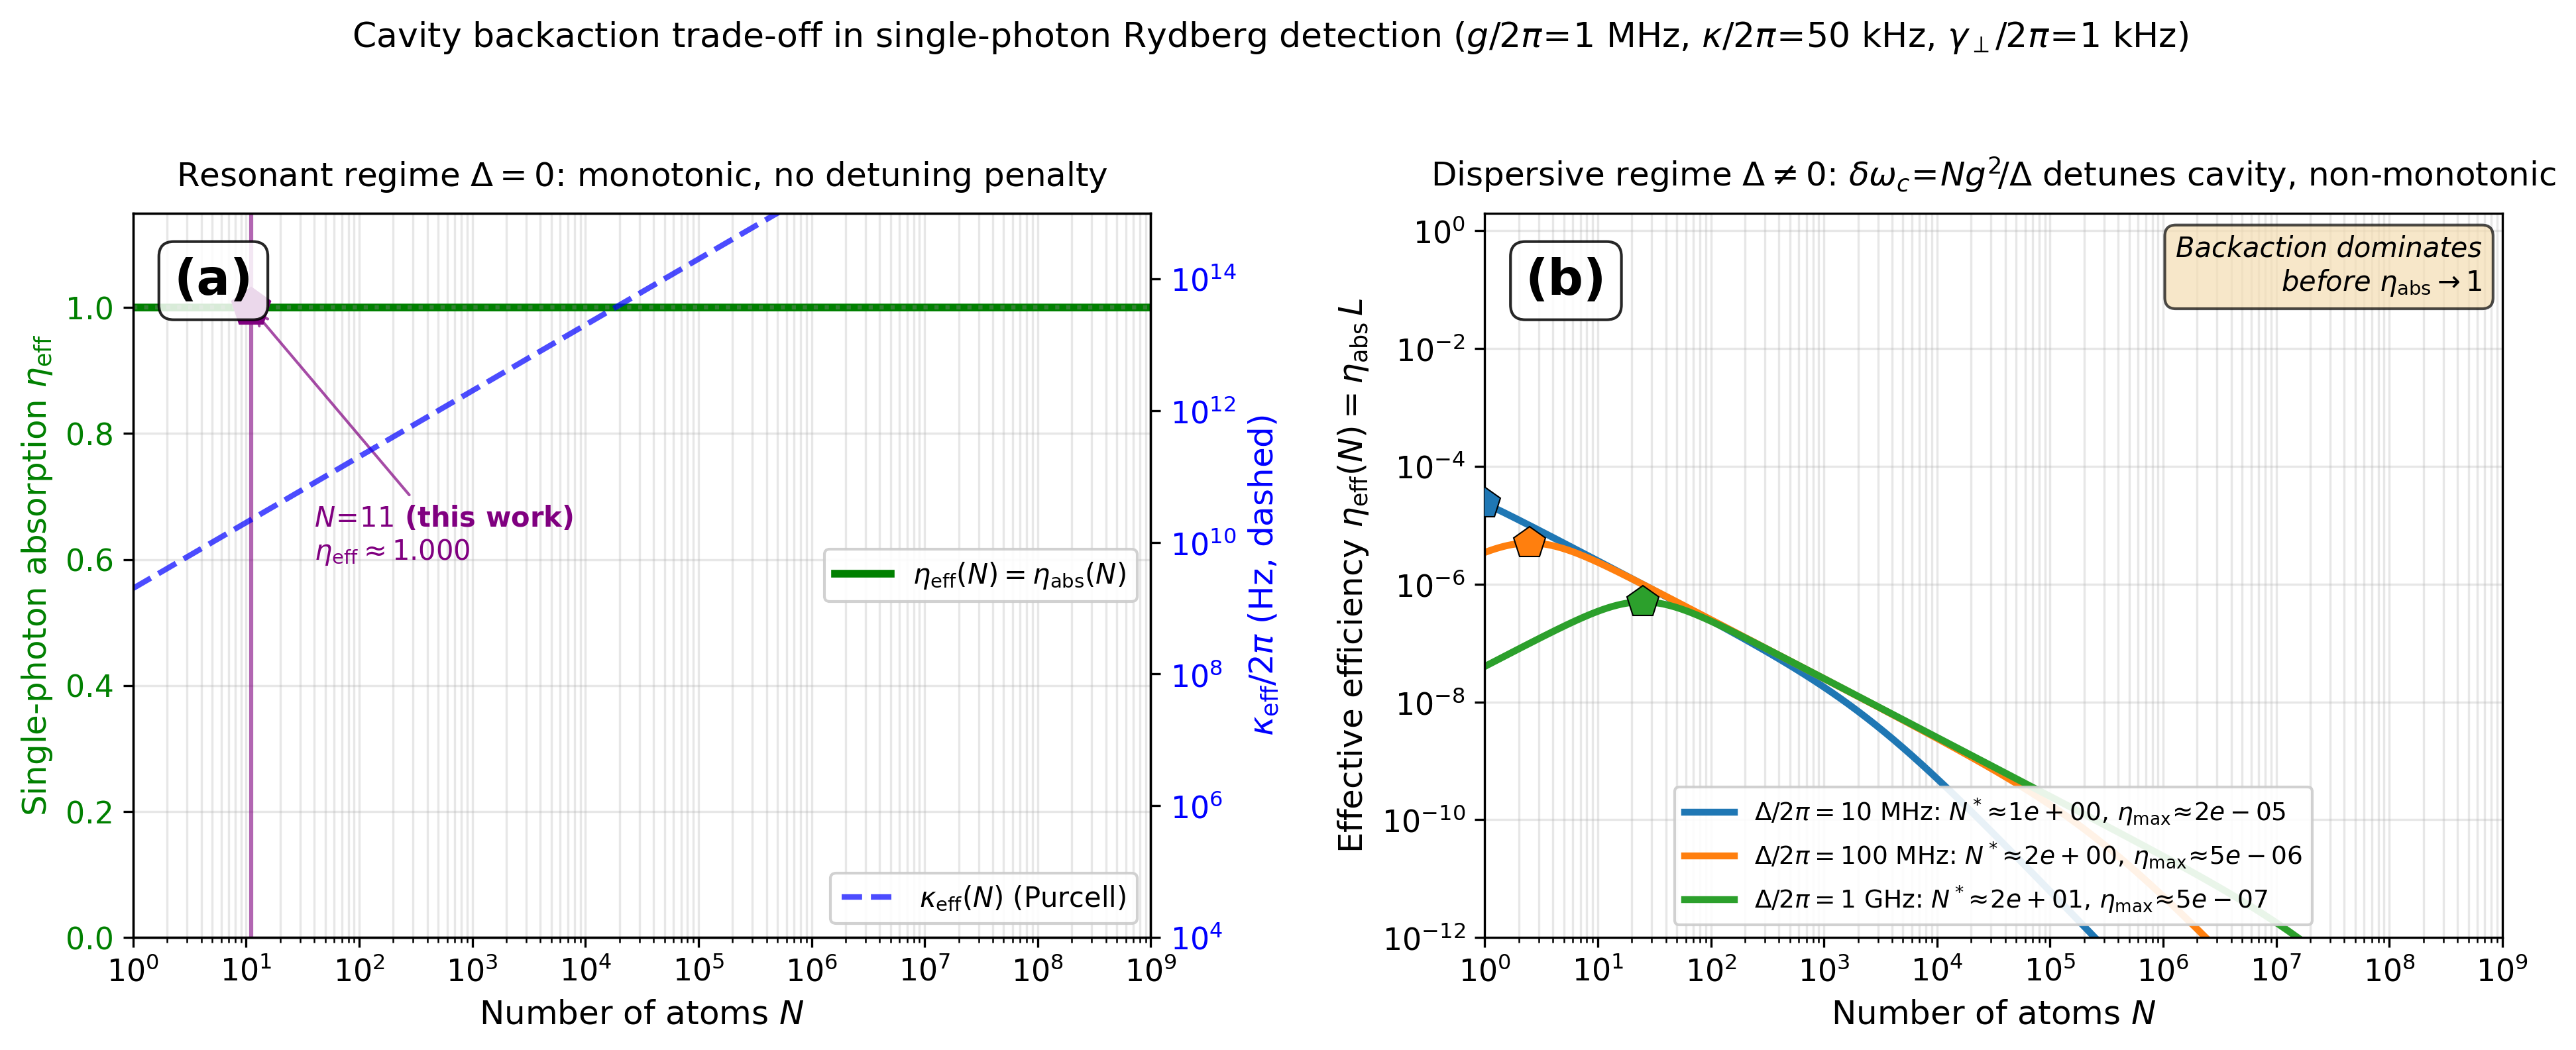
\includegraphics[width=\textwidth]{chapters/qs_figures/backaction_eta_eff_vs_N.png}
    \caption{Effect of cavity backaction on the single-photon detection efficiency $\eta_{\rm eff}(N)$. \textbf{(a)} Resonant regime ($\Delta = 0$): $\eta_{\rm eff}^{\rm res}(N) = 2C/(1+2C)$ is monotonic and saturates to unity already at $N = \mathcal{O}(1)$ for the parameters considered (single-atom cooperativity $C_1 \approx 2\!\times\!10^4$); the only consequence of large $N$ is the Purcell broadening of the cavity linewidth $\kappa_{\rm eff}(N) = \kappa\,[1\!+\!2C(N)]$ (right axis, dashed blue). The working point of this thesis ($N=11$, purple) sits comfortably in the saturated regime. \textbf{(b)} Dispersive regime ($\Delta \neq 0$): the cavity dispersive shift $\delta\omega_c\!=\!Ng^2/\Delta$ detunes the cavity from the axion-photon resonance, applying a Lorentzian penalty $L(N)$ to the absorbed signal. The product $\eta_{\rm eff}^{\rm disp}(N) = \eta_{\rm abs}(N)\,L(N)$ is non-monotonic and admits a finite optimum $N^*$, but the peak efficiency $\lesssim\!2\times10^{-5}$ remains too small for practical detection regardless of the choice of detuning $\Delta$. The conclusion is that the resonant configuration is the natural architectural choice for high-efficiency single-photon haloscope readout.}
    \label{fig:backaction}
\end{figure}

This backaction analysis closes the loop on a concern that naturally arises for ensembles of this size: the multi-atom avalanche scheme studied here does not suffer from the dispersive-regime sensitivity penalty because, by construction, the atomic transition is tuned on resonance with the cavity, and the cooperativity of the resonant scheme is already in the deeply saturated regime at $N=11$. Larger ensemble sizes ($N\!\sim\!100$ and beyond) would not improve the single-photon coupling efficiency, and their practical role would be limited to providing a longer effective avalanche chain---an option already discussed at the level of facilitation dynamics in Sec.~\ref{sec:scalability_atoms}.

\subsubsection*{Cryogenic Operation}

While the detector operates at $4$~K, the surrounding cavity and magnet may require lower temperatures for optimal performance. A staged cooling architecture is envisioned: the atomic platform at the $4$~K pulse-tube stage, the cavity at an optional $1$~K $^4$He pot stage, and the cavity together with the HEMT amplifiers at a $300$~mK $^3$He stage.

This approach balances detector performance (lower $T$ reduces dark counts) with system complexity.

\section{Scalability}
\label{sec:scalability_atoms}

The amplification factor $\mathcal{A} \sim N$ suggests that larger systems provide greater sensitivity. However, several factors may impact scalability.

\subsubsection{Hilbert Space Growth}

The exact quantum simulation scales exponentially as $\mathcal{O}(2^N)$ in memory and $\mathcal{O}(2^N \cdot N_{\rm steps})$ in time for sparse-Hamiltonian evolution. In practice we have performed direct sesolve simulations up to $N = 17$ atoms ($2^{17} \approx 1.3 \times 10^5$ basis states, $\sim 200$~MB peak memory, $\sim 1$~h walltime per magnetic-field point on a single CPU core); $N = 19$ remains tractable but with a runtime of several hours. Beyond $N \gtrsim 21$ approximate methods such as matrix product states or truncated Wigner approximations are required, exploiting the one-dimensional geometry and weak-excitation regime. Hardware limitations ultimately necessitate experimental validation. Simulation on quantum computing systems could also be explored.

\subsubsection{Decoherence}

Real systems experience decoherence from three main mechanisms: spontaneous emission with rate $\Gamma_{\mathrm{sp}} \sim 1/n^3$ (microseconds for $n \sim 70$), dephasing due to laser phase noise and trap intensity fluctuations, and collisional decoherence, suppressed at low density and temperature.

Our simulations assume coherent evolution over timescales $T_a \sim 10$ $\mu$s, which is achievable given typical Rydberg lifetimes $> 100$ $\mu$s. Inclusion of decoherence effects would reduce the amplification factor but not eliminate it entirely; systematic studies~\cite{Festa2022} suggest that avalanche amplification is robust to moderate decoherence rates.

\subsubsection{Optimal System Size}

There exists an optimal system size $N^*$ that maximises detection efficiency while maintaining coherence. Based on the theoretical analysis of Ref.~\cite{Nill2024}, we estimate $N^* \sim 10$--20 atoms for typical experimental parameters. Beyond this, the benefits of increased amplification are offset by larger decoherence and readout complexity.

\subsection*{Frequency Range}

The detector resonance is not the binding energy of the Rydberg state (which
is of order meV, i.e.\ sub-THz, and sets instead the field-ionisation and
thermal-robustness scales discussed above) but the frequency of the
dipole-allowed transition between the two Rydberg states addressed by the
axion-converted photon,
\begin{equation}
    f = \frac{E_{n'} - E_{n}}{h}
    \;\approx\; \frac{2\,\mathrm{Ry}}{h\, n_{\rm eff}^{3}}
    \qquad (\Delta n = 1),
\end{equation}
which scales as $n^{-3}$. For rubidium, adjacent-manifold transitions give
\begin{itemize}
    \item $n = 50$: $f \approx 64$ GHz ($\sim 260~\mu$eV axions)
    \item $n = 70$: $f \approx 22$ GHz ($\sim 90~\mu$eV axions)
    \item $n = 100$: $f \approx 7$ GHz ($\sim 30~\mu$eV axions)
\end{itemize}
while $\Delta n = 0$ pairs split only by the quantum-defect difference
(e.g.\ $nS \to nP$) lie a factor of $\sim 2$--$4$ lower at the same $n$,
extending the accessible band to a few GHz for $n \gtrsim 90$. Together
with higher-$\Delta n$ transitions, this tunability enables coverage of a
substantial part of the QCD axion mass window ($1$--$1000~\mu$eV) with a
single detector platform, a significant advantage over fixed-frequency
superconducting detectors.

\section{Detection-fidelity caveats and modelling assumptions}

Several limitations of the current approach merit discussion:

\subsubsection{Detection Fidelity}
\label{sec:detection_fidelity}

The simulations presented in this chapter compute the true Rydberg population $S(t)$ as a function of time. To translate this microscopic observable into a single-shot detection statement, two distinct conditions must be assessed: (i) the click count produced by the realistic readout chain must be statistically separable from the dark-count background at a chosen confidence level, and (ii) the same click count must exceed the detection threshold $S_{\rm thr}$ with the desired probability when an axion-induced avalanche has actually occurred. These two criteria are independent and we evaluate them in turn.

\paragraph{Dark-count rejection.}
For an array of $N=11$ atoms at $T = 4$~K, the thermal excitation rate is $N\Gamma_{\rm thermal} \sim 1.1 \times 10^{-2}$~Hz (Eq.~\eqref{eq:thermal_rate_total}). The natural detection window is the avalanche timescale $T_a \approx 9$~$\mu$s, so the expected number of thermally-induced Rydberg excitations per shot is $\langle n_{\rm dark, true}\rangle = N\Gamma_{\rm thermal}T_a \sim 10^{-7}$. Even after attenuation by the detection efficiency, the expected number of dark-count clicks per shot remains well below $10^{-7}$. Assuming Poisson statistics, the probability of a single spurious click triggering a false detection is therefore
\begin{equation}
    P(\text{false positive}) = 1 - e^{-\eta_{\rm det} N \Gamma_{\rm thermal} T_a} \approx \eta_{\rm det} N \Gamma_{\rm thermal} T_a \sim 10^{-7},
\end{equation}
which sits five orders of magnitude below the $3\sigma$ rejection threshold of $2.7 \times 10^{-3}$. Any threshold $S_{\rm thr} \geq 1$ click therefore satisfies $3\sigma$ background rejection by an enormous margin, irrespective of the choice of readout. Dark-count rejection is not a limiting factor of the present scheme; the cryogenic operating temperature has already done the work.

\paragraph{Single-shot detection probability.}
The non-trivial criterion is the second one: given that an avalanche has actually been triggered by a converted photon, the number of recorded clicks must exceed $S_{\rm thr}$ with probability $\geq 1 - 2.7 \times 10^{-3}$ (the formal $3\sigma$ level). With $S_{\rm thr} = 1$ click, the detection probability under Poisson statistics is
\begin{equation}
    P(\text{detect}\,|\,\text{signal}) = 1 - e^{-\eta_{\rm det} \mathcal{A}},
    \label{eq:detection_probability}
\end{equation}
and the $3\sigma$ condition reduces to $\eta_{\rm det}\mathcal{A} > \ln(1/2.7\times 10^{-3}) \approx 5.92$ expected clicks. This is a quantitative requirement on the product of amplification factor and readout efficiency.

To map the trade-off between these two factors we have repeated the avalanche simulation at $N = 11, 13, 15, 17$ for all four magnetic-field operating points ($B = 0, 1, 3, 5$~T), and fitted the resulting amplification factors with a linear model $\mathcal{A}(N) = a + bN$. The results, shown in Fig.~\ref{fig:N_scaling}(a), give $a = 2.31$ and $b = 0.286$. The linear form $\mathcal{A} \propto N$ reproduces the signal scaling $\mathcal{S} \propto N$ established for this protocol by Nill~\emph{et al.}~\cite{Nill2024}, who showed that during the ballistic phase the Rydberg-excitation number grows linearly in time up to the optimal amplification time $T_a \propto N/\Omega_{\rm gr}$. The slope is significantly below the naive mean-field expectation $b \sim 1/2$: the avalanche front sweeps the whole one-dimensional chain within $T_a \sim N/\Omega_{\rm gr}$ and saturates, while dephasing among already-excited sites further suppresses the propagation efficiency. This anomalous-percolation behaviour is consistent with the regime characterised experimentally in bulk Rydberg gases~\cite{Helmrich2020, Wintermantel2021} and analysed theoretically by Brady~\emph{et al.}~\cite{Brady2024}.

\begin{figure}[ht]
    \centering
    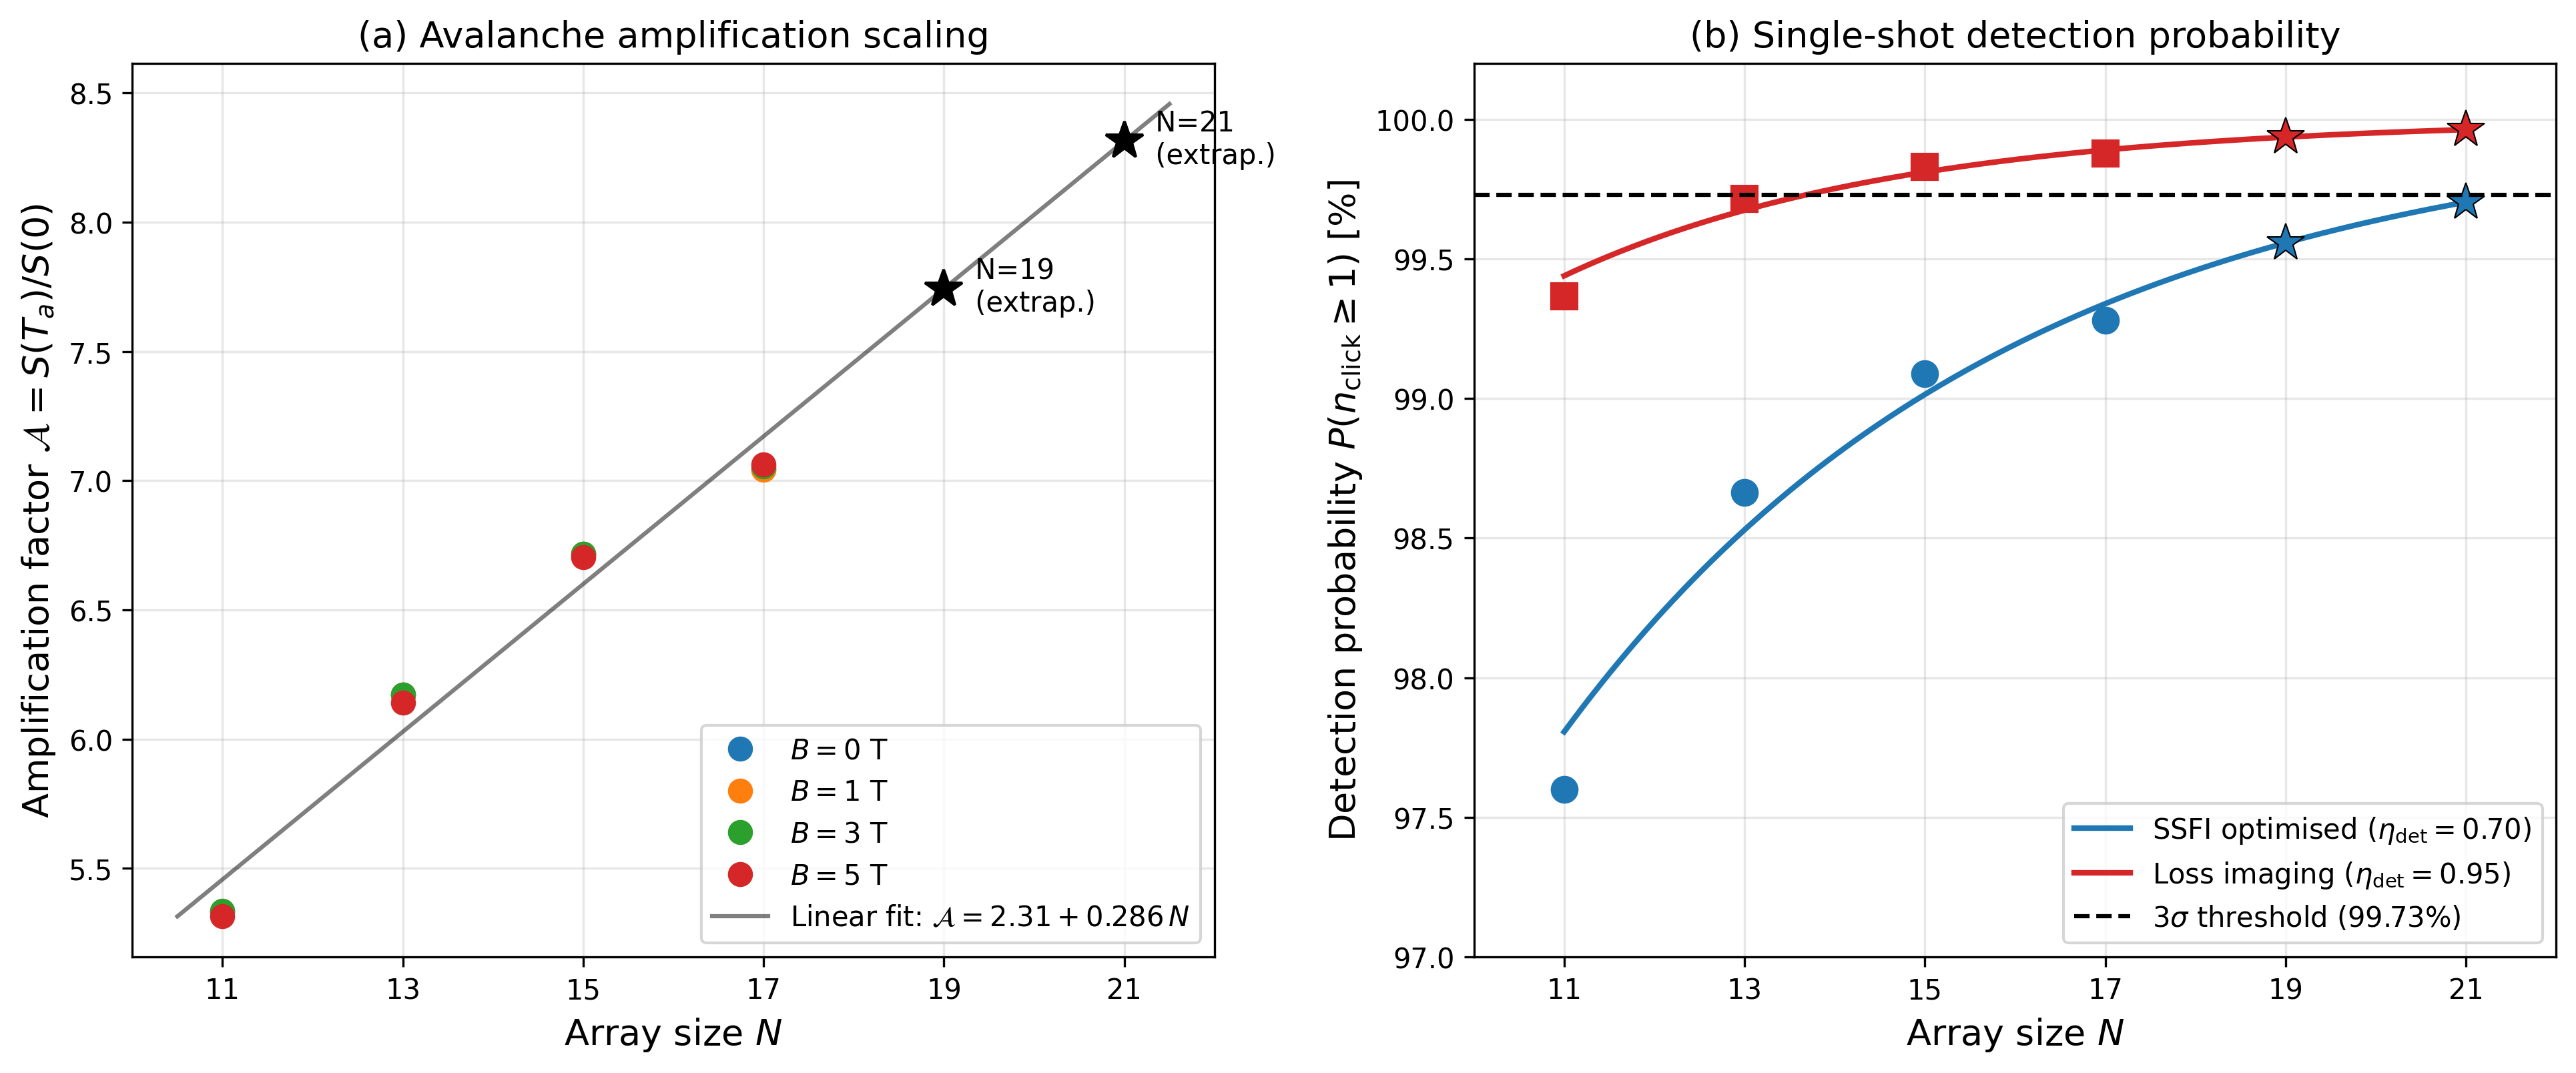
\includegraphics[width=\textwidth]{chapters/qs_figures/amplification_vs_N.png}
    \caption{Avalanche amplification scaling with array size and resulting detection probability. \textbf{(a)} Amplification factor $\mathcal{A} = S(T_a)/S(0)$ as a function of the array size $N$ for the four magnetic-field values $B = 0, 1, 3, 5$~T. Coloured circles are simulated points; black stars at $N = 19, 21$ are the linear extrapolation of the fit $\mathcal{A}(N) = 2.31 + 0.286\,N$ (grey line). The four $B$ values overlap to within $1\%$ at every $N$, confirming that the auto-detuning protocol keeps the facilitation condition exactly satisfied across the haloscope-relevant field range. The slope $b = 0.286$ is below the naive mean-field prediction $b \sim 1/2$: the avalanche front traverses the whole one-dimensional chain within $T_a$ and saturates, with dephasing among already-excited sites further reducing the propagation efficiency. \textbf{(b)} Single-shot detection probability $P(n_{\rm click} \geq 1)$ as a function of $N$, for the two readout strategies considered (state-selective field ionisation at $\eta_{\rm det} = 0.70$, blue; loss imaging at $\eta_{\rm det} = 0.95$, red). Solid curves use $\mathcal{A}(N)$ from the linear fit; circles and squares mark the simulated points; stars mark the extrapolated points at $N = 19, 21$. The dashed black line is the formal $3\sigma$ threshold (99.73\%). Loss imaging crosses the threshold already at $N = 15$ via direct simulation; SSFI does not cross within the simulated range and would require $N \gtrsim 23$ according to the linear extrapolation.}
    \label{fig:N_scaling}
\end{figure}

The two readout technologies relevant to the present scheme are state-selective field ionisation (SSFI) and loss imaging. They are based on fundamentally different physical mechanisms and operate at opposite ends of the efficiency--complexity trade-off. We describe each in turn.

\paragraph{State-selective field ionisation (SSFI).}
This is the standard readout technique in cold-Rydberg experiments~\cite{Gallagher2005, Saffman2016}, in which the Rydberg atoms are detected through their own ionisation rather than through optical interaction with the ground state. The protocol exploits the fact that the outer electron of a Rydberg atom is bound by only a few meV, so that a moderate static or pulsed electric field is sufficient to ionise it. The ionisation field for a state of principal quantum number $n$ scales as $E_{\rm cr} \sim 3.2 \times 10^8 / n_{\rm eff}^4$~V/cm, where $n_{\rm eff} = n - \delta_\ell$ accounts for the quantum defect $\delta_\ell$~\cite{Gallagher2005}. For the principal quantum numbers of interest here ($n \sim 70$, $n_{\rm eff} \approx 65$--$67$), critical fields of order $15$~V/cm are sufficient. Operationally, after the avalanche has completed its dynamics, a ramp of electric field is applied to the array via planar or cylindrical electrodes; atoms in the targeted Rydberg state ionise with essentially unit probability~\cite{Ryabtsev2007} as soon as the ramp crosses $E_{\rm cr}$, and the freed ions (or, equivalently, electrons) are directed to a microchannel-plate (MCP) detector. Because the ionisation threshold $E_{\rm cr}$ depends sharply on $n$, an appropriately tuned ramp slew rate provides spectral resolution between adjacent Rydberg manifolds, which is the origin of the ``state-selective'' qualifier~\cite{Tada1999}. The end-to-end detection efficiency is set by the product of three loss factors: the MCP collection efficiency (set by the electrostatic optics that guide the charged particles, typically $60$--$80\%$), the MCP quantum efficiency (set by the secondary-electron yield of the first plate at the impact energy chosen, typically $60$--$80\%$ for keV ions or electrons), and incidental losses from collisional ionisation, off-resonant decay during the ramp, or non-ideal selectivity ($1$--$5\%$). In state-of-the-art implementations the product yields $\eta_{\rm det} \approx 40$--$70\%$~\cite{Ryabtsev2007, Andersen2013}, with the upper end of the range corresponding to dedicated geometries optimised for single-atom resolution; preliminary results from chip-integrated SSFI~\cite{Seery2024} suggest that further improvement is possible in highly engineered settings. The technique is intrinsically destructive on the atomic state, since each detection event annihilates a Rydberg atom and ejects an ion; this is not a problem for axion-haloscope operation, where each detection cycle is a separate shot, but it imposes the limit that the same atomic ensemble cannot be re-interrogated within a single avalanche event.

\paragraph{Loss imaging.}
This technique is widely used in modern tweezer arrays for ground-state qubit readout~\cite{Endres2016, Bluvstein2024} and is applied to Rydberg detection by reversing the question: rather than detecting the Rydberg atoms themselves, one detects the \emph{absence} of those atoms from their original tweezer sites. A short ``blowout'' step is applied first --- this can be a rapid field-ionisation pulse, a Rydberg-to-untrapped-state transfer via microwave, or a resonant push beam --- and removes every Rydberg atom from the trap with near-unit efficiency. A subsequent fluorescence-imaging step then images the ground-state atoms that remained in place via a closed cycling transition; the absence of fluorescence at a site that was loaded before the avalanche indicates that the atom was promoted to a Rydberg state, while sites where fluorescence is recovered indicate atoms that remained in the ground state throughout. All detection losses are therefore confined to the single photon-scattering step on the ground-state transition, where modern implementations achieve site-discrimination fidelities of $99.97\%$ on $10^4$ lattice sites~\cite{Tao2024} and $99.99\%$ on arrays of $6\,100$ atoms~\cite{Manetsch2025}, with imaging-induced atom loss in the $0.01\%$ range. The end-to-end efficiency $\eta_{\rm det} \geq 95\%$ used in this chapter is therefore conservative with respect to the current state of the art. The price paid for this gain in efficiency is a more complex experimental sequence: an additional blowout pulse with accurate calibration of the depletion fidelity (any residual Rydberg population that is not removed introduces a systematic offset in the count), an imaging beam with low-noise camera optics, and the requirement that the tweezer positions be stable on the timescale of the imaging exposure. None of these is a fundamental obstacle, and several proposals~\cite{Bluvstein2024, Manetsch2025} have demonstrated integrated tweezer-imaging architectures consistent with the Rydberg-haloscope geometry envisioned here.

Figure~\ref{fig:N_scaling}(b) shows the detection probability as a function of $N$ for both readout strategies, using $\mathcal{A}(N)$ from the linear fit. With optimised SSFI ($\eta_{\rm det} = 0.70$) the detection probability rises from $97.6\%$ at $N=11$ to $99.3\%$ at $N=17$ (simulated), and the linear extrapolation predicts $99.70\%$ at $N=21$ --- still marginally below the $3\sigma$ threshold of $99.73\%$. Crossing the formal $3\sigma$ threshold within the SSFI strategy would require $N \gtrsim 23$, a regime outside the present computational budget; the curvature visible in panel~(b) further suggests that the linear extrapolation is not conservative. SSFI is therefore a viable readout for the present scheme but does not, by itself, suffice for $3\sigma$-confident single-shot single-photon detection.

The optimal readout for the present scheme is loss imaging. With $\eta_{\rm det} = 0.95$ the detection probability reaches $99.83\%$ at $N = 15$, a value obtained from direct simulation (no extrapolation), comfortably above the $3\sigma$ threshold. Loss imaging combined with $N = 15$ atoms is therefore the minimal-resource configuration that achieves $3\sigma$ single-shot single-photon detection in the present scheme.

It is important to emphasise that this conclusion concerns only the \emph{readout} stage: the avalanche dynamics, the facilitation condition, the auto-detuning protocol, and the spatiotemporal correlations analysed in the preceding sections are independent of the detection technology. The two readout options bracket a continuous range of performance trade-offs that an experimental implementation may navigate.

\subsubsection{One-Dimensional Geometry}

Our simulations assume a 1D atomic chain. Extension to 2D or 3D geometries would increase the coordination number, giving each atom more facilitation pathways but also more configurations in which an atom borders two or more excited neighbours and is pushed off resonance by the antiblockade shift. Whether the net effect enhances or suppresses $\mathcal{A}$ relative to the 1D chain is not determined by the present analysis and would require avalanche simulations on higher-dimensional lattices with a finite-size scaling study. The proposal of Ref.~\cite{Nill2024} also considers 2D extensions of the avalanche scheme, suggesting this generalisation is feasible in principle, although still awaiting experimental confirmation.

\subsubsection{Photon Absorption Efficiency}

We have assumed perfect absorption of cavity photons by the atomic ensemble. In reality, the absorption efficiency is given by:

\begin{equation}
    \eta_{\mathrm{abs}} = \frac{N \Gamma_{\mathrm{abs}}}{\kappa + N \Gamma_{\mathrm{abs}}}
\end{equation}

where $\Gamma_{\mathrm{abs}} = g^2/\Gamma_{\mathrm{sp}}$ is the single-atom absorption rate, $g$ is the atom-cavity coupling, and $\kappa$ is the cavity decay rate. Realistic cavity-atom coupling parameters ($g \sim 2\pi \times 1$~MHz, $\kappa \sim 2\pi \times 0.05$~MHz) yield $\eta_{\mathrm{abs}} \sim 0.5$--$0.8$ for $N=11$ atoms. This reduces the effective detection efficiency but does not affect the single-photon sensitivity claim. For strong coupling ($g \gg \kappa, \Gamma_{\mathrm{sp}}$) and large $N$, near-unity efficiency is still possible~\cite{Hogan2012}.

\subsubsection{Single-Shot vs. Integrated Detection}

The simulations model the single-shot detection of individual photons. In practice, axion experiments integrate over long times ($\sim 100$ s) to accumulate signal. The avalanche detector must be reset after each detection cycle, limiting the maximum detection rate to $\sim 1/(T_a + T_{\mathrm{reset}}) \sim 10$ kHz. For the axion photon rates relevant here, $R_\gamma\!\sim\!\mathcal{O}(10)$--$\mathcal{O}(10^2)$~s$^{-1}$ (cf.\ Eq.~\ref{eq:photon_rate}), this maximum detection rate is more than adequate.

\section{Alternative Rydberg Detection Schemes}

The avalanche amplification approach studied here is one of several potential Rydberg-based detection schemes. Other possibilities include:

\subsubsection{Electromagnetically Induced Transparency (EIT)}

Rydberg EIT enables the detection of microwave photons via changes in probe laser transmission~\cite {Holloway2014}. This approach offers high sensitivity and has been demonstrated at room temperature; however, it lacks the amplification provided by avalanche dynamics.

\subsubsection{Rydberg Superheterodyne Receiver}

By mixing the microwave signal with a local oscillator, the detection frequency can be downconverted to an intermediate frequency where conventional amplifiers operate more efficiently~\cite{Jing2020}. This approach may complement avalanche detection in a hybrid architecture.

\subsubsection{Rydberg Excitons in Cuprous Oxide}

Recent work~\cite{Gallagher2022,Walther2024} has explored the use of Rydberg excitons in the semiconductor Cu$_2$O as solid-state analogues of Rydberg atoms. These systems offer the advantage of compact, cryogenic-compatible platforms but face challenges from disorder and phonon coupling. Extension of avalanche amplification to this platform remains an open question.

\section{Comparison with Other Platforms}
Rydberg sensors complement superconducting and solid-state platforms with two distinct operating regimes: Rydberg \emph{electrometers}, based on EIT readout, operate at room temperature and offer wide spectral tunability for field sensing, while the \emph{photon-counting} architecture studied in this chapter is operated cryogenically (4~K) to suppress blackbody-induced dark counts. SQUIDs achieve unmatched magnetic sensitivity but require liquid-helium (4~K) cryogenics and have limited frequency range. NV centres operate at room temperature with modest magnetic sensitivity. Table~\ref{tab:compare} summarises their comparative attributes.

\begin{table}[htbp]
\centering
\caption{Comparison between selected quantum sensing platforms.}
\begin{tabular}{lccc}
\toprule
Platform & Temperature & Sensitivity & Bandwidth \\
\midrule
SQUID & 4~K & fT/$\sqrt{Hz}$ & kHz--MHz \\
NV centre & 300~K & nT/$\sqrt{Hz}$ & MHz \\
Rydberg atom (photon detection, this work) & 4~K & $\sim 10^{-22}$ W & Hz-THz \\
Rydberg atom (field sensing, EIT) & 300~K & $<1~\mu$V/cm/$\sqrt{Hz}$ & Hz--THz \\
Trapped ion & 4~K & nT/$\sqrt{Hz}$ & Hz--kHz \\
\bottomrule
\end{tabular}
\label{tab:compare}
\end{table}

Quantum sensors increasingly form part of hybrid systems, combining quantum front-ends with classical control and learning-based inference. In future architectures, distributed Rydberg sensors could read out superconducting qubits at the quantum limit, linking sensing and computation in integrated quantum networks~\cite{Ezratty2024}.

%==============================================================================
\section{Conclusions}
\label{sec:axion_conclusions}

We have presented a theoretical investigation of Rydberg avalanche amplification as a candidate single-photon detector for axion-haloscope readout. The numerical simulations of this chapter indicate that the scheme combines single-photon sensitivity ($\sim 10^{-22}$~W), low background ($< 0.01$~Hz at 4~K), and compatibility with strong magnetic fields (0--5~T), three requirements that have so far been difficult to satisfy simultaneously in a single haloscope-compatible detector.

\subsection*{Summary of findings}

The amplification factor at $N=11$ atoms is $\mathcal{A} \approx 5.3$, and remains essentially constant as the external magnetic field is scanned from $0$ to $5$~T, with the four sampled field values overlapping to within $1\%$ at every $N$ in the range examined. Direct simulation at $N = 11, 13, 15, 17$ establishes a linear scaling $\mathcal{A}(N) = 2.31 + 0.286\,N$ that holds uniformly across the same field range; the underlying mechanism is the laser auto-detuning, which absorbs the Zeeman shift of the driven transition and preserves the facilitation condition. The thermal background, exponentially suppressed in $\Delta E/k_BT$, falls below $0.01$~Hz at $T = 4$~K and below $10^{-4}$~Hz at $T = 300$~mK; these figures sit in the range demonstrated for the leading superconducting single-photon technologies operated at sub-Kelvin temperatures, and the present analysis suggests that they remain accessible at the $4$~K operating point examined here.

The avalanche timescale is $T_a \sim 10~\mu$s, approximately an order of magnitude shorter than the typical Rydberg-state radiative lifetime at $n\sim 70$ ($\sim 100~\mu$s, Ref.~\cite{Beterov2009}), so the coherent regime modelled in this chapter is the relevant operating regime in practice. A full Lindblad treatment of pure dephasing has not been performed here and is left to follow-up work; systematic studies of comparable facilitation schemes~\cite{Festa2022} report that the amplification mechanism is not fragile to moderate dephasing on the timescale of a single avalanche event. The avalanche additionally produces a V-shaped spatial signature in the excitation density that provides an internal discriminator against background events, as discussed in Sec.~\ref{sec:axion_benchmarking}. State-selective field ionisation, the standard detection technique for cold Rydberg atoms~\cite{Gallagher2005, Saffman2016}, has demonstrated end-to-end efficiencies $\eta_{\rm det} \approx 40$--$70\%$~\cite{Ryabtsev2007, Andersen2013}, sufficient to deliver a single-shot detection probability of $99.3\%$ at $N=17$ in our simulations; loss imaging at $\eta_{\rm det} \geq 95\%$~\cite{Tao2024, Manetsch2025} reaches $P_{\rm detect} = 99.83\%$ at $N=15$ and would satisfy the formal $3\sigma$ threshold. The choice between the two readouts is an experimental design parameter; the avalanche physics analysed in this chapter is independent of either.

Operationally, the principal quantum number $n$ provides a tuning knob: varying $n$ shifts the resonant frequency, so a single experimental platform can in principle address axion masses across the range from approximately $1~\mu$eV to $1$~meV (GHz to THz frequencies) without redesigning the hardware. The combined parameter space --- single-photon sensitivity, operation in multi-tesla magnetic fields, low thermal background, and $4$~K operating temperature --- addresses several of the constraints that have made photon counting in the haloscope context difficult to satisfy with a single detector; whether this combination translates into experimentally useful sensitivity will depend on details of the integration with a conversion cavity that are outside the scope of this chapter.

\subsection*{Outlook}

The model developed here is a starting point, not an experimental result. Several steps would be needed before the predictions of this chapter could be tested against a working detector. Integrating a cold-Rydberg platform with a cryogenic microwave cavity is the first of these, both because it determines whether the optical access required for trapping and readout is compatible with the cavity geometry, and because cavity losses and photon-injection coupling enter the detection efficiency directly. A demonstration of the avalanche amplification in the presence of magnetic fields up to $5$--$7$~T would then test the central prediction of the present analysis. Characterisation of dark count rates under realistic experimental conditions, measurement of photon absorption efficiency, and the development of single-atom imaging techniques compatible with cryogenic and high-field environments are the natural follow-ups; none of them is a small undertaking on its own, and the predictions of this chapter would have to be revisited as data become available.

 The treatment developed in this chapter is coherent (unitary), and on that basis it establishes four results: the facilitation-driven amplification mechanism and its leading-order magnitude ($\mathcal{A}\approx5.3$ at $N=11$, scaling as $\mathcal{A}=2.31+0.286\,N$); the field-independence of the amplification across $0$--$5$~T, which follows from the laser auto-detuning at the level of the Hamiltonian and is therefore insensitive to dissipation; the ballistic avalanche timescale $T_a\sim N/\Omega_{\mathrm{gr}}$ and the V-shaped spatial signature; and the single-shot detection probabilities with the associated array-size thresholds for $3\sigma$ confidence. A full Lindblad treatment, including pure dephasing and radiative decay, would add four results that the present analysis can only bound or infer from the literature: a quantitative dephasing correction turning $\mathcal{A}\approx5.3$ from a coherent upper bound into a realistic value at finite $T_2$; the dephasing rate ($\Gamma_\phi T_a\sim1$) at which the coherent--ballistic picture crosses over to the classical, directed-percolation regime characterised experimentally in driven Rydberg gases~\cite{Helmrich2020}; a self-consistent account of radiative and blackbody-induced decay during the avalanche; and a robustness curve $\mathcal{A}(\Gamma_\phi)$ in place of the qualitative robustness inferred from comparable facilitation experiments~\cite{Festa2022}. Such a study would refine the present predictions downward and delimit their regime of validity, while leaving unchanged the field-independence and the dark-count budget, neither of which is sensitive to the coherent-versus-dissipative distinction.

Beyond the axion-haloscope context, the detection scheme analysed here may also be relevant to microwave-regime quantum communication, sensitive RF sensing for radar and radio astronomy, searches for other weakly coupled particles such as dark photons or chameleons, and tests of fundamental physics in cavity-QED settings. These applications share the requirement of single-photon sensitivity in regimes where the standard superconducting detectors do not operate naturally; whether the scheme of this chapter is competitive in any of them is a question that the present work does not address.

\section*{Acknowledgments}

The author acknowledges the use of the QuTiP library for quantum simulations~\cite{Johansson2013,qutip5}. This work builds on the foundational theoretical proposal of Ref.~\cite{Nill2024}, predicting terahertz avalanche detection in Rydberg atoms.




